\documentclass[12pt,draftcls,peerreview,onecolumn]{IEEEtran}
%\documentclass[10pt,conference,twocolumn]{IEEEtran}
%\documentclass[10pt,conference]{IEEEtran}
\usepackage{epsf}
\usepackage{amsmath,amssymb}
\usepackage{graphicx}
\usepackage{color}
\usepackage{cite}
\usepackage{multirow,tabularx}
\usepackage{ifthen}
% Add these after the document class declaration
\usepackage{times}
\usepackage{stackrel}
%\usepackage{hyperref}
\usepackage{enumerate}
\graphicspath{{./plots/}}
%\input{epsf.sty}
%\pagestyle{bfheadings}
%-------------------------------

%\input{commands.tex}

\renewcommand{\baselinestretch}{1.65}
\newcommand{\showfigure}{\boolean{true}}
%\newcommand{\showfigure}{\boolean{false}}

\newcommand{\hide}[1]{\ifthenelse{\boolean{false}}{#1}{}}

%\include{../../commonHeader}
%%%%%%%%%%%%%%%%%%%%%%
% Theorems, etc.

\newtheorem{theorem}{{\bf Theorem}}
\newtheorem{lemma}{{\bf Lemma}}
\newtheorem{proposition}[theorem]{Proposition}
\newtheorem{corollary}{{\bf Corollary}}
\newtheorem{result}{{\bf Result}}

%\newenvironment{proof}[1][Proof]{\begin{trivlist}
%\item[\hskip \labelsep {\bfseries #1}]}{\end{trivlist}}

%\newtheorem{defn}{Definition}
\newenvironment{definition}[1][Definition]{\begin{trivlist}
\item[\hskip \labelsep {\bfseries #1}]}{\end{trivlist}}

\newenvironment{example}[1][Example]{\begin{trivlist}
\item[\hskip \labelsep {\bfseries #1}]}{\end{trivlist}}

\newenvironment{remark}[1][Remark]{\begin{trivlist}
\item[\hskip \labelsep {\bfseries #1}]}{\end{trivlist}}

\newcommand{\qed}{\nobreak \ifvmode \relax \else
      \ifdim\lastskip<1.5em \hskip-\lastskip
      \hskip1.5em plus0em minus0.5em \fi \nobreak
      \vrule height0.75em width0.5em depth0.25em\fi}


\newtheorem{fact}{Fact}
\newtheorem{obs}{Observation}

%%%%%%%%%%%%%%%%%%%%%%
% Environments

\newcommand{\barr}{\begin{array}}
\newcommand{\earr}{\end{array}}



%%%%%%%%%%%%%%%%%%%%%%
% References

\newcommand{\eqn}[1]{(\ref{#1})}

%%%%%%%%%%%%%%%%%%%%%%
% Brackets

\newcommand{\brac}[1]{\left({#1}\right)}
\newcommand{\sbrac}[1]{\left[{#1}\right]}
\newcommand{\cbrac}[1]{\left\{{#1}\right\}}

\newcommand{\floor}[1]{\left\lfloor{#1}\right\rfloor}

%%%%%%%%%%%%%%%%%%%%%%
% Misc

\newcommand{\expc}[2][]{E_{#1}\left[{#2}\right]}

\newcommand{\set}[1]{\{#1\}}

\newcommand{\ul}{\underline}
\newcommand{\smq}[1]{{\it #1}}
\newcommand{\ave}[1]{\overline{#1}}

\newcommand{\recip}[1]{\frac{1}{{#1}}}

%%%%%%%%%%%%%%%%%%%%%%
% Indicator function

\newcommand{\indic}[1]{I_{\cbrac{#1}}}

%%%%%%%%%%%%%%%%%%%%%%
% Superscripts
\newcommand{\supth}{^{{\mathrm{th}}}}
\newcommand{\mth}{^{{\mathrm{th}}}}
\newcommand{\supnd}{^{{\mathrm{nd}}}}
\newcommand{\suprd}{^{{\mathrm{rd}}}}


%%%%%%%%%%%%%%%%%%%%%%
% Combinatorics

\newcommand{\nchoosek}[2]{\left(\begin{array}{c}
                                {#1} \\ {#2}
                             \end{array}
                        \right)}

%%%%%%%%%%%%%%%%%%%%%%
% Symbols
\newcommand{\CN}{{\cal CN}}
\newcommand{\db}{{\mathrm dB}}
\newcommand{\Om}{\widehat{\Omega}}

\newcommand{\define}{\triangleq}
%\newcommand{\define}{\stackrel{\triangle}{=}}
%\newcommand{\implies}{\Rightarrow}
%\newcommand{\tendsto}{\rightarrow}
\newcommand{\tendsto}{\to}

\newcommand{\degree}{^{\circ}}
\newcommand{\kroneck}{\otimes}

%%%%%%%%%%%%%%%%%%%%%%
% Special phrases

\newcommand{\ie}{{i.e.}}
\newcommand{\eg}{{e.g.}}
\newcommand{\etal}{{et al.}}
\newcommand{\wrt}{w.r.t.}
\newcommand{\vs}{{vs.}}

%%%%%%%%%%%%%%%%%%%%%%
% Matrix related

\newcommand{\tvec}{\text{vec}} % \vec is already defined
\newcommand{\mtx}[1]{{\bf #1}} % matrix
\newcommand{\mtxg}[1]{{\boldsymbol #1}} % matrix for greek symbol

\newcommand{\trp}{\text{T}} % transpose
\newcommand{\trc}[1]{\text{Tr}\left\{{#1}\right\}} % trace

%%%%%%%%%%%%%%%%%%%%%%
% Special matrices


\newcommand{\mzero}{\mtx{0}}

%%%%%%%%%%%%%%%%%%%%%%
% Principal sub-matrix

\newcommand{\princ}[2]{{#2}^{({#1})}}
\newcommand{\princsup}[3]{{{#2}^{({#1})^{#3}}}}

%%%%%%%%%%%%%%%%%%%%%%
% Probability related

\newcommand{\EX}{\bf{E}} % expectation operator
\newcommand{\expect}[1]{{\bf{E}}\left[{#1}\right]}
\newcommand{\expectpow}[2]{{\bf{E}}^{#2}\left[{#1}\right]}
\newcommand{\explow}[2]{{\bf{E}}_{#1}\left[{#2}\right]}
\newcommand{\prob}[1]{\text{Pr}\brac{#1}}
\newcommand{\pr}{{\text{Pr}}}

%%%%%%%%%%%%%%%%%%%%%%
% Derivatives

\newcommand{\deriv}[2]{\frac{d{#1}}{d{#2}}}
\newcommand{\pderiv}[2]{\frac{\partial{#1}}{\partial{#2}}}

%%%%%%%%%%%%%%%%%%%%%%
% Slides

\newcommand{\bsp}{\begin{slide*}}
\newcommand{\esp}{\end{slide*}}
\newcommand{\bsl}{\begin{slide}}
\newcommand{\esl}{\end{slide}}
\newcommand{\vsp}[1]{\vspace{#1}}





%-------------------------------
% This paper's specific shortcuts

\newcommand{\nbm}[1]{{[\bf nbm: #1]}}
\newcommand{\vinod}[1]{[\textsl{v: #1}]}
\newcommand{\var}[1]{{\bf var}\left[{#1}\right]}
\newcommand{\opt}{\text{opt}}
\newcommand{\sth}{\text{th}}

\DeclareMathOperator*{\argmin}{arg\,min}
\DeclareMathOperator*{\argmax}{arg\,max}
%\newcommand{\var}{var}

\newcommand{\dv}{D}
\newcommand{\newdv}{{\cal D}^{\prime}}

\newcommand{\abs}[1]{\left\lvert{#1}\right\lvert}

%\newcommand{\err}{\text{Err}}

\newcommand{\given}{\arrowvert}
\newcommand{\givens}{\big\arrowvert}
\newcommand{\Given}{\Big\arrowvert}

\newcommand{\bMQAM}{b_{\text{QAM}}}
\newcommand{\bMPSK}{b_{\text{PSK}}}

\newcommand{\cMPSK}{c_{\text{PSK}}}
\newcommand{\cMQAM}{c_{\text{QAM}}}

%\newcommand{\opt}{\text{opt}}
%\newcommand{\asym}{\text{asm}}


%\newcommand{\err}{\text{Err}}


%% \newcommand{\alphaoptasm}{\alpha_{\opt}^{\asym}}
%% \newcommand{\betaoptasm}{\beta_{\opt}^{\asym}}


%\newcommand{\sepMPSK}{P_{\text{MPSK}}}

\newcommand{\limgamma}{\lim_{\gamma \tendsto \infty}}


\newcommand{\SEP}{\text{SEP}}
\newcommand{\SEPdouble}{\text{SEP}_{\text{si}}}


\newcommand{\sinpiM}{\sin^2\brac{\frac{\pi}{M}}}

\IEEEoverridecommandlockouts
\newcommand{\ceil}[1]{\left\lceil{#1}\right\rceil}

\newcommand{\est}[1]{\widehat{#1}}

\newcommand{\y}{\mathbf{y}}


\newcommand{\hg}{\mathbf{hg}}
\newcommand{\nx}{{0}}
%\newcommand{\nck}[2]{{{#1}\choose{#2}}}
\newcommand{\nck}[2]{\binom{#1}{#2}}
\newcommand{\setA}{A}
\newcommand{\setAk}{\setA_{k}}
\newcommand{\setB}{B_k}


\newcommand{\setAkhat}{\widehat{\setA}_k}

%\newcommand{\setAone}{\!\gk{1}\!>\!\taubypt,\setB\!}
\newcommand{\setG}{G}
\newcommand{\setL}{L}
\newcommand{\setGk}{\setG_k}
\newcommand{\setLk}{\setL_k}

\newcommand{\setGkhat}{\widehat{\setG}_k}
\newcommand{\setLkhat}{\widehat{\setL}_k}

\newcommand{\setBgk}{B_{gk}}
\newcommand{\setBlk}{B_{lk}}


\newcommand{\snh}{\sin^2(\theta)} 
\newcommand{\onebysin}{\frac{1}{\sin^2(\theta)}} 

\newcommand{\bg}{\frac{\be}{\ga}}
\newcommand{\twobg}{\frac{2\be}{\ga}}
\newcommand{\be}{\alpha}

\newcommand{\ginc}[2]{\gamma\left({#1},{#2}\right)}
\newcommand{\gincnew}[2]{\widetilde{\gamma}\left({#1},{#2}\right)}


\newcommand{\lam}{\lambda}
\newcommand{\lamstar}{\lam^{*}}
\newcommand{\lamp}{\lam_{p}}
\newcommand{\lamasym}{\lam_{\text{a}}}
\newcommand{\lamub}{\lam_{\text{ub}}}
\newcommand{\lsg}{{\lam\mg}}
\newcommand{\s}[1][]{s_{#1}}
\newcommand{\sphi}{s}
%\newcommand{\sphi}{s_{\phi}}

\newcommand{\slam}{s_{\lam}}
\newcommand{\szero}{s_{0}}
\newcommand{\sstar}{s^{*}}
\newcommand{\shp}{s_{h}}
\newcommand{\ipi}{{\frac{1}{\pi}}}
\newcommand{\intmpi}{{\int_{0}^{\zerosep\pi}}}
\newcommand{\intm}{{\int_{0}^{\zerosep}}}
\newcommand{\intinf}{{\int_{0}^{\infty}}}
\newcommand{\intg}{{\int_{0}^{\frac{\zerosep-y_1}{\lam}}}}

\newcommand{\error}{\epsilon_n} 

\newcommand{\mug}{{\mu_{g}}}

\newcommand{\muh}{{\mu_{h}}}

\newcommand{\yg}[1]{y_{#1}+\lam g_{#1}}


\newcommand{\Err}{{\text{Err}}}

\newcommand{\z}{{\cal{Z}}}
\newcommand{\tL}{{L}}
\newcommand{\K}{{\left(1+\frac{\mh}{\eta\mg}\right)}}
\newcommand{\M}{{\left(\frac{\eta\mg}{\eta\mg+\mh}\right)}}
\newcommand{\prlseta}{{\left(\frac{\eta\mg}{\eta\mg+\mh}\right)}}
\newcommand{\frhg}[1]{{\frac{h_{#1}}{g_{#1}}}}
\newcommand{\pdfh}{{\frac{e^{-\frac{h_1}{\mh}}}{\mh}}}
\newcommand{\pdfg}{{\frac{e^{-\frac{g_1}{\mg}}}{\mg}}}\newcommand{\frM}{{\frac{\mg h_1}{\mh g_1+\mg h_1}}}



\newcommand{\MPSKSEP}{\exp\brac{\frac{-h_1\Et\sinpiM}{\sigma^2\sin^2\theta}}}

\newcommand{\F}{\cal{F}}
\newcommand{\goodset}{\cal{G}}
\newcommand{\badset}{\cal{B}}
\newcommand{\setc}{\cal{C}}
\newcommand{\setszero}{{\cal{S}}_0}
\newcommand{\setonegt}{{\cal{S}}_{11}}

\newcommand{\setonelt}{{\cal{S}}_{12}}
\newcommand{\MI}{\text{MI}}
\newcommand{\MSLIR}{\text{MSLIR}}

\newcommand{\termone}{T_1}
\newcommand{\termtwo}{T_2}

\newcommand{\Nt}{{N_t}}
\newcommand{\Nr}{{N_r}}
\newcommand{\Np}{{N_p}}
\newcommand{\Pt}{{P_t}}


\newcommand{\such}{h}
\newcommand{\puch}{g}


\newcommand{\hk}[1]{{\such_{#1}}}
\newcommand{\gk}[1]{{\puch_{#1}}}


\newcommand{\hi}{\hk{i}}
\newcommand{\gi}{\gk{i}}

\newcommand{\hij}{{\such_{ij}}}
\newcommand{\gkj}{{\puch_{kj}}}

\newcommand{\selp}{s_{p}}
\newcommand{\sopt}{s^{*}}

\newcommand{\h}{\mathbf{\such}}
\newcommand{\g}{\mathbf{\puch}}


\newcommand{\ghatvec}{\mathbf{\hat{\puch}}}
\newcommand{\yhatvec}{\mathbf{\hat{y}}}

\newcommand{\Rsrx}{R_{i}}
\newcommand{\Iprx}{I_{p}}
\newcommand{\Isrx}{I_{i}}

\newcommand{\noise}{n_i}

\newcommand{\noisevar}{\sigma^2}

\newcommand{\outsym}{\out_{\text{asym}}}
\newcommand{\outhp}{\out_{{h}}}
\newcommand{\outwb}{\out_{\text{wub}}}
\newcommand{\prout}{\prob{\text{out}}}
\newcommand{\outmax}{O_{\text{max}}}
\newcommand{\itau}{\tau}
\newcommand{\ibeta}{\beta}

\newcommand{\cone}{c_{1}}
\newcommand{\ctwo}{c_{2}}
\newcommand{\cthree}{c_{3}}
\newcommand{\cfour}{c_{4}}

\newcommand{\out}{O}
%\newcommand{\m}{\cone}

\newcommand{\outmaxhrule}{e^{-\taubyptmug}}
\newcommand{\taubyptmug}{\frac{\itau}{\mug\Pt}}
\newcommand{\Nttaubyptmug}{\frac{\Nt\itau}{\mug\Pt}}
\newcommand{\taubypt}{\frac{\itau}{\Pt}}
\newcommand{\gkgrtaubypt}[1]{{\gk{#1}}>\taubypt}
\newcommand{\gklttaubypt}[1]{{\gk{#1}}\leq\taubypt}

\newcommand{\gkhatgrtaubypt}[1]{{\gkhat{#1}}>\taubypt}
\newcommand{\gkhatlttaubypt}[1]{{\gkhat{#1}}\leq\taubypt}



\newcommand{\gindic}[1]{\indic{\gkgrtaubypt{#1}}}
\newcommand{\ghatindic}[1]{\indic{\gkhatgrtaubypt{#1}}}

\newcommand{\lambym}{\frac{\lam}{\cone}}

\newcommand{\lamstarbym}{\frac{\lamstar}{\cone}}


\newcommand{\yk}[1]{y_{#1}}
\newcommand{\ykplambym}[1]{\yk{#1}+\lambym}
\newcommand{\xplambym}{x+\lambym}
\newcommand{\ccdfyray}[1]{\left(1-\left(#1\right)^{\albysnr[]}\right)}
\newcommand{\sepg}[1]{\SEP(\hk{#1}) + \lam \gindic{#1}}
\newcommand{\ykplusgk}[1]{ \yk{#1} + \lambym\gindic{#1}}
\newcommand{\ykhatplusgkhat}[1]{ \ykhat{#1} + \lambym\ghatindic{#1}}
\newcommand{\ccdfg}[1][]{e^{-\frac{{#1}\itau}{\mug\Pt}}}
\newcommand{\inlccdfg}[1][]{\exp\left({-{{#1}\itau}/{\left( \mug\Pt\right) }}\right)}


\newcommand{\ai}{a}
\newcommand{\bj}{b}
\newcommand{\cj}{c}
\newcommand{\outopt}{\out_{\text{opt}}}
\newcommand{\lamopt}{\lam_{\text{opt}}}

\newcommand{\inty}{\int_{0}^{1-\lambym}}
\newcommand{\al}{\ctwo}
\newcommand{\snr}{\Omega}
\newcommand{\Ptmuhbynoisevar}{\frac{\Pt\muh}{\noisevar}}
\newcommand{\albysnr}[1][]{\frac{\al#1}{\snr}}
\newcommand{\snrbyal}[1][]{\frac{\snr#1}{\al}}



\newcommand{\un}{U}
\newcommand{\prggrtaubyp}{e^{-\taubyptmug}}
\newcommand{\prggrNttaubyp}{e^{-\Nttaubyptmug}}
\newcommand{\probszero}{\un\left(1-\left(1-\lambym\right)^{\albysnr[]}\right)^{\Nt}}


\newcommand{\allopts}{\left\{\nx,1,\ldots,\Nt\right\}}
\newcommand{\antopts}{\left\{1,2,\ldots,\Nt\right\}}
\newcommand{\twoopts}{\left\{2,\ldots,\Nt\right\}}


\newcommand{\nropts}{\left\{1,2,\ldots,\Nr\right\}}
\newcommand{\puopts}{\left\{1,2,\ldots,\Np\right\}}

\newcommand{\maxh}{{\text{best antenna}}}
\newcommand{\ub}{{\text{UB optimal}}}
\newcommand{\IIC}{{\text{IIC}}}
\newcommand{\iic}{{\text{iic}}}
\newcommand{\EIIC}{{\text{Gamma}}}
\newcommand{\eiic}{{\text{gamma}}}

\newcommand{\mi}{{\text{mi}}}
\newcommand{\mslir}{{\text{mslir}}}
\newcommand{\emi}{\text{emi}}
\newcommand{\emslir}{\text{emslir}}
\newcommand{\interfUncons}{I_{\text{un}}}
\newcommand{\sepUBL}{\SEP^{(\tL)}_{UB}}
\newcommand{\sepUBTwo}{\SEP^{(2)}_{UB}}
\newcommand{\interfUnconsMI}{I_{\text{unmi}}}
\newcommand{\DS}{\text{ds}}
\newcommand{\rBeta}{{\text{Beta}}}
\newcommand{\rbeta}{{\text{beta}}}
\newcommand{\igamma}{{\frac{\al\noisevar}{\Pt}\ln\left(\frac{1}{1-\left(\lam/\cone\right) }\right)}}
\newcommand{\igammainline}{{- \left( {\al\noisevar}/{\Pt}\right)  \ln\left({1-\lam/\cone }\right) }}

\newcommand{\suchph}{\theta}
\newcommand{\puchph}{\varphi}

\newcommand{\thetahk}{\suchph_{is}}
\newcommand{\thetagk}{\puchph_{s}}

\newcommand{\asrule}{\phi}
\newcommand{\asspan}{{\cal A}}
\newcommand{\feasrule}{\phi}
\newcommand{\phiprop}{\phi_{p}}

\newcommand{\psifun}[2]{\psi_{{#1},{#2}}}
%\newcommand{\psifun}[2]{\psi_{k_1k_2}\left({#1},{#2}\right)}

\newcommand{\onemlc}{\left[1-\lambym\right]}
%\newcommand{\onemlc}{\left(\!\frac{\cone\!-\!\lam}{\cone}\!\right)}

\newcommand{\thresh}{\beta}
\newcommand{\sg}{s_{\igamma}}
\newcommand{\og}{\out_{\igamma}}

%\newcommand{\zerosep}{\left(1 - \frac{1}{M}\right)}
\newcommand{\zerosep}{e_0}

\newcommand{\Hmx}{\mtx{H}}
\newcommand{\Gmx}{\mtx{G}}


\newcommand{\ith}{i^{\text{th}}}
\newcommand{\jth}{j^{\text{th}}}
\newcommand{\kth}{k^{\text{th}}}

\newcommand{\optproblem}{{\cal P}}

\newcommand{\caluncons}{{\cal S_{\text{0}}}}
\newcommand{\callamrule}{{\cal S_{{\lam}}}}
\newcommand{\outlam}{\out_{\lam}}
\newcommand{\outhatlam}{\widehat{\out}_{\lam}}
\newcommand{\outhatlamstar}{\widehat{\out}_{\lam^*}}
\newcommand{\outUBlam}{\out_{\text{UB}\lam}}
\newcommand{\outUBtwo}{\out_{\text{UB2}}}
\newcommand{\callamstarrule}{\cal S_{\lam^{*}}}

\newcommand{\calhprule}{{\cal S_{\text{h}}}}

\newcommand{\avgSEP}{\overline{\SEP}}

\newcommand{\akone}{\albysnr[k_1]}
\newcommand{\jidx}{j}

\newcommand{\nullset}{\varnothing}


% imperfect CSI related commands

\newcommand{\sug}{\alpha}
\newcommand{\pug}{\beta}

\newcommand{\sugain}[1]{\sug_{#1}}
\newcommand{\pugain}[1]{\pug_{#1}}

\newcommand{\sugainhat}[1]{\widehat{\sug}_{#1}}
\newcommand{\pugainhat}[1]{\widehat{\pug}_{#1}}

\newcommand{\unhat}{\widehat{\un}}
\newcommand{\snrhat}{\widehat{\snr}}

\newcommand{\gpilotpower}{P_g}
\newcommand{\hpilotpower}{P_h}

\newcommand{\hhat}{\hat{\such}}
\newcommand{\ghat}{\hat{\puch}}
\newcommand{\yhat}{\hat{y}}
\newcommand{\shat}{\hat{s}}

\newcommand{\hkhat}[1]{\hhat_{#1}}
\newcommand{\gkhat}[1]{\ghat_{#1}}
\newcommand{\ykhat}[1]{\hat{y}_{#1}}


\newcommand{\muhhat}{\mu_{\hhat}}
\newcommand{\mughat}{\mu_{\ghat}}

\newcommand{\ccdfghat}[1][]{e^{-\frac{{#1}\itau}{\mughat\Pt}}}
\newcommand{\ccdfghatinline}{\exp\left( {-{\itau}/{\left( \mughat\Pt\right) }}\right) }

\newcommand{\Probglt}{B}

\newcommand{\albysnrhat}[1][]{\frac{\al#1}{\snrhat}}
\newcommand{\snrhatbyal}[1][]{\frac{\snrhat#1}{\al}}

\newcommand{\rhog}{\rho_g}
\newcommand{\rhoh}{\rho_h}

\newcommand{\Tc}{\frac{1}{\snrhatbyal\left(1 + \snrbyal\left(1 - \rhoh \right)  \right) }}

%\newcommand{\Dc}{\frac{1 + \snrbyal}{\snrhatbyal\left(1 + \snrbyal\left(1 - \rhoh \right)  \right) }-1}

\newcommand{\T}{\varpi}
\newcommand{\Dc}{\T \left( 1 + \snrbyal\right) -1}

\newcommand{\hpilotsym}{x_{s}}
\newcommand{\gpilotsym}{x_{p}}

\newcommand{\hpilotrcv}{y_{ik}}
\newcommand{\gpilotrcv}{z_{k}}

\newcommand{\hpilotnoise}{n_{ik}}
\newcommand{\gpilotnoise}{n_{k}}

\newcommand{\ccdfyNr}[1]{\frac{\gamma\left(\Nr,-\albysnr\ln{#1}\right)}{(\Nr-1)!}} 
\newcommand{\unccdfy}[2]{\frac{{#1}\,\,\gamma\left(\Nr,-\albysnr\ln{#2}\right)}{(\Nr-1)!}}

\newcommand{\pdfyNr}{\frac{\left(\albysnr\right)^{\Nr}\left(-\ln\left({x}\right)\right)^{\Nr-1}x^{\albysnr[]-1}}{(\Nr-1)!}} % only y terms constants taken care separately
\newcommand{\ytimespdfyNr}{\left(\ln\left(\frac{1}{x}\right)\right)^{\Nr-1}x^{\albysnr[]}} % only y terms constants taken care separately
\newcommand{\ypluslamtimespdfyNr}{\left(\ln\left(\frac{1}{x+\lambym}\right)\right)^{\Nr-1}\left(x+\lambym\right)^{\albysnr[]}} % only y terms constants taken care separately


\newcommand{\pdfyNrgen}[1]{f_{y}\left(#1\right)} % only y terms constants taken care separately
\newcommand{\ccdfy}[1]{F^{c}_{y}\left(#1 \right)}
\newcommand{\unccdfygen}[2]{{#1} \ccdfy{#2}  }

\newcommand{\ccdfyrv}[1]{ F^{c}_{y}\left(#1 \right) }
\newcommand{\ccdfyhatrv}[1]{F^{c}_{\yhat}\left(#1 \right) }
\newcommand{\pdfy}[1]{ f_{y}\left( #1 \right) }
\newcommand{\pdfyhat}[1]{f_{\yhat}\left( #1 \right) }

\newcommand{\Xhat}{\widehat{X}}
\newcommand{\xhat}{\hat{x}}


\newcommand{\sumnr}{\sum_{i=1}^{\Nr}}




\begin{document}

\title{Transmit Antenna Selection for Interference-Outage Constrained Underlay CR}

\author{Rimalapudi Sarvendranath, {\it Student Member, IEEE}, Neelesh B. Mehta, {\it Senior Member, IEEE}}

\author{
	Rimalapudi Sarvendranath, {\it Student Member, IEEE}, Neelesh B. Mehta, {\it Senior Member, IEEE}
	
	\thanks{Rimalapudi Sarvendranath and Neelesh B.\ Mehta are with the
		Dept.\ of Electrical Communication Eng.\ at the Indian Institute of
		Science (IISc), Bangalore, India. Emails:
		sarvendranath@gmail.com, nbmehta@iisc.ac.in}
		\thanks{A part of this paper has been accepted for presentation in the IEEE Global
		Communications Conf. (Globecom), Singapore, Dec. 2017~\cite{sarvnedranath_2017_globecom}.}
}

\setcounter{page}{1}

\maketitle

\begin{abstract}
Transmit antenna selection (TAS) is a low hardware complexity technique that improves the performance of an interference-constrained underlay cognitive radio (CR) system by exploiting spatial diversity. We propose a novel TAS rule called the $\lambda$-weighted interference indicator rule (LWIIR). We prove that it is optimal in terms of minimizing the average symbol error probability (SEP) of an underlay CR system that is subject to the interference-outage constraint. This constraint imposes a limit on the probability that the interference power at the primary exceeds a threshold. It is a generalization of the widely studied peak interference constraint, and is practically well motivated. We derive the average SEP of LWIIR for any given number of transmit and receive antennas. The rule and its performance analysis apply to a general class of fading models with continuous distributions and to many constellations. We also analyze the practically important scenario in which the secondary transmitter has imperfect information of the channel gains from itself to the secondary and primary receivers. We show that the imperfections in these two sets of channel gains have different impacts on the system. Our extensive benchmarking shows that LWIIR markedly outperforms many selection rules considered in the literature.

\end{abstract}


\begin{IEEEkeywords}
Cognitive radio, underlay, antenna selection, interference-outage constraint, symbol error probability, imperfect CSI.
\end{IEEEkeywords}

\IEEEpeerreviewmaketitle



\section{Introduction}	
\label{sec:intro}

Cognitive radio (CR) technology has the potential to mitigate the scarcity of radio spectrum by enabling different classes of users to access the spectrum together without an exclusive and inefficient allocation of the spectrum to just one class of users~\cite{Goldsmith_2009_PIEEE}. Owing to its promise, it has been incorporated in IEEE standards such as 802.11af and 802.22~\cite{Sherman_2008_TCMAG}, and continues to attract considerable attention. In CR, users are classified into two categories, namely,   primary users (PUs), who are licensed users of the spectrum, and  secondary users (SUs), who are unlicensed users of the same spectrum. The following three modes of access have been investigated for CR~\cite{Goldsmith_2009_PIEEE}: (i)~Interweave mode, in which an SU can only transmit in unused time or frequency resources, (ii)~Overlay mode, in which SU has access to the data and channel gains of the  PU and can transmit simultaneously with it, and (iii)~Underlay mode, in which an SU can transmit concurrently in the same spectrum as the PU, but must ensure that the interference due to its transmissions to the primary receiver (PRx) is below a tolerable limit. 

In this paper, we focus on underlay CR as it enables frequency reuse~\cite{Zhang_2017_tcom} by allowing for a controlled amount of interference to the primary and has received considerable attention in the literature~\cite{Hanif_2015_globecom,Wang_2010_TWC,RZhang_2009_TWC,Sarvendranath_2013_TCOM,Wang_2011_TCom,Sarvendranath_2014_TCOM, Kashyap_2014_TCOM,Kong_2011_JCN,Fakhan_2014_TSP,Hanif_2017_tcom,Sboui_2013_TWC,Kashyap_2015_wicomlet,li_2011_pimrc}. Furthermore, in the time division duplexing (TDD) mode of operation, an SU can exploit reciprocity and operate in the underlay CR mode based on periodic measurements of the primary signal and does not require extensive coordination with the primary. The performance of underlay CR is fundamentally governed by the constraint imposed on the interference caused to the PRx. 

Various interference constraints have been investigated in the literature. These include: (i)~Peak interference constraint~\cite{Fakhan_2014_TSP,Hanif_2015_globecom,Wang_2010_TWC,RZhang_2009_TWC,Suraweera_2010_TVT,li_2011_pimrc}, in which  the instantaneous interference power at the PRx cannot exceed  a threshold; (ii)~Average interference constraint~\cite{ Sarvendranath_2013_TCOM,Sarvendranath_2014_TCOM,Wang_2011_TCom}, in which  the fading-averaged interference power at the PRx  cannot exceed  a threshold;  and (iii)~Interference-outage constraint~\cite{Kashyap_2014_TCOM,Sboui_2013_TWC}, in which the event that the interference exceeds a certain value is referred to as an interference-outage, and the probability of an interference-outage cannot exceed a threshold. Among these constraints, the peak interference constraint is the one that has received the most attention in the underlay CR literature. However, as we see from above, it is only one among many possible constraints. 

These interference constraints can significantly limit the performance of the secondary system. This has spurred the investigation of advanced techniques to improve the secondary system performance. Transmit antenna selection (TAS) is an important example of this. It exploits the spatial diversity afforded by multiple antennas while avoiding the hardware complexity of the latter~\cite{mehta_2012_ComMag}. Only one radio frequency (RF) chain, which is dynamically switched to one of the antennas based on the current channel conditions, is required. 

%Given its benefits, TAS has attracted considerable attention in the underlay CR literature~\cite{Dmochowski_2011_CROWNCOM,Wang_2011_TCom,Hanif_2015_globecom,Sarvendranath_2013_TCOM,Wang_2010_TWC,Kong_2011_JCN}.
Compared to a single antenna system, TAS can significantly improve the ergodic capacity of the secondary,~\cite{Hanif_2015_globecom,Wang_2010_TWC}, and reduce the secondary outage probability~\cite{Hanif_2015_globecom,Kong_2011_JCN} and symbol error probability (SEP)~\cite{Sarvendranath_2013_TCOM,Sarvendranath_2014_TCOM} at the secondary receiver (SRx), or increase the outage capacity~\cite{Kong_2011_JCN}. In TAS for underlay CR, the choice of the antenna at the secondary transmitter (STx) is driven not just by the channel gains from it to the SRx's antenna(s), but also by the interference it causes to the PRx. It also crucially depends on the interference constraint imposed on the secondary system. %In recognition of this, the following different TAS rules, which specify the antenna to be selected as a function of the instantaneous channel gains, have been considered in the literature. 
In recognition of this, we restrict our focus only to the literature related to TAS for the above interference constraints. The following different TAS rules, which specify the antenna to be selected as a function of the instantaneous channel gains, have been considered in the literature
%
\begin{itemize}
\item {\em Peak Interference Constraint:} In~\cite{Hanif_2015_globecom}, among the antennas that satisfy the peak interference constraint, the one with the highest STx to SRx (STx-SRx) channel power gain is selected. It is easy to show that this maximizes the SU rate or minimizes the SEP for a fixed transmit power model. Instead, in~\cite{Wang_2010_TWC}, for an  STx that transmits with a power inversely proportional to the STx to PRx (STx-PRx) channel power gain, the antenna with the highest ratio of the STx-SRx and STx-PRx channel power gains is selected. 
%
\item {\em Average Interference Constraint:} A difference TAS rule is proposed in~\cite{Wang_2011_TCom}, which selects the antenna with a maximum weighted difference of the STx-SRx and STx-PRx channel power gains. For an STx that transmits with fixed power, in~\cite{Sarvendranath_2013_TCOM}, an optimal TAS rule that minimizes the average SEP is proposed. %It is shown that the optimal antenna is one that minimizes a linear combination of the STx-PRx channel power gain and an exponentially decreasing function of the STx-SRx channel power gain. 
This model was extended to include power adaptation in~\cite{Sarvendranath_2014_TCOM}. %Furthermore, for an STx that adapts its transmit power, in~\cite{Sarvendranath_2014_TCOM}, an average SEP optimal TAS rule is proposed. It is shown that optimal antenna is one that maximizes the ratio of STx-SRx channel power gain and an affine combination of the STx-PRx channel power gain and a constant. 
%
\item{\em Interference-Outage Constraint:} To the best of our knowledge, no TAS rule has been studied for this constraint, and the optimal TAS rule is not known in the literature. However, we note that~\cite{Peng_2016_eurasip} proposed an ad hoc power back-off technique to control interference-outage at the primary with imperfect channel state information (CSI) at the STx.

\end{itemize}


In this paper, we focus on the interference-outage constraint given that it has been less investigated even though it is theoretically and practically well motivated.  Firstly, it is a generalization of the extensively studied peak interference constraint, which corresponds to the extreme case in which the interference-outage probability is zero. Therefore, a more general class of underlay CR systems is covered by this constraint. Furthermore, the peak interference constraint cannot be met without perfect  CSI of the instantaneous STx-PRx channel power gain at the STx, which is difficult to ensure in practice~\cite{musavian_2009_tcom,Suraweera_2010_TVT,Peng_2016_eurasip}. Secondly, as mentioned, the optimal TAS rule for it is not known in the literature, and it cannot be inferred from the TAS rules proposed for the other interference constraints. Thirdly, in terms of the impact on the primary system, this constraint is justified when the primary offers delay or disruption tolerant services, or the primary traffic is based on user datagram protocol (UDP) services like voice and video traffic. Furthermore, it need not be disruptive to the primary wireless systems, which are already designed to tolerate deep fades or co-channel interference. 

\subsection{Contributions} 
We make the following contributions in this paper:
\begin{itemize}
\item We first propose a novel TAS rule called the $\lam$-weighted interference indicator rule (LWIIR) for an interference-outage constrained %multiple input multiple output (MIMO) 
underlay CR system. It selects the antenna that minimizes a sum of two terms. The first term is the instantaneous SEP of that antenna and the second term is the indicator function of STx-PRx channel power gain weighted by an interference-outage penalty factor $\lam$. To the best of our knowledge, such a rule has not been proposed in the literature and differs from those in~\cite{Wang_2011_TCom,Dmochowski_2011_CROWNCOM,Wang_2010_TWC}.

\item We prove that LWIIR has the following optimality property among all the TAS rules that satisfy the interference-outage constraint.  For a general class of fading models with a continuous cumulative distribution function (CDF), which we shall henceforth refer to as the {\em continuous fading model}, it yields the lowest fading-averaged SEP for the secondary system. We note that the average SEP is an important measure of reliability, and has been studied in the related literature~\cite{Fakhan_2014_TSP,Kashyap_2014_TCOM,Sarvendranath_2013_TCOM,Sarvendranath_2014_TCOM,li_2011_pimrc,Suraweera_2010_TVT}. 

%
\item We then analyze the average SEP of LWIIR. First, we derive a general expression that is in a single integral form for any fading model and for an arbitrary number of receive antennas at the SRx. We gain several insights about its behavior by considering various special cases of interest. We show that it simplifies to an insightful closed-form for Rayleigh fading with SRx having one antenna. %These average SEP expressions provide valuable insights into its behavior with different parameters, unlike brute force simulations based approach. 
Our extensive benchmarking results bring out the significant reductions in the average SEP achieved by LWIIR compared to ad hoc adaptations of the rules considered in the literature. 
% 
\item We derive a novel integral-free upper bound on the interference-outage probability of LWIIR. This further leads us to an insightful and tight closed-form upper bound for $\lam$.
% 
%\item We also show that in high transmit power region the optimal rule transforms into a very simple form. This results in a closed-form exact expression for interference-outage probability.       
%
%\item To gain further insights, we derive a simpler upper bound on the interference-outage probability for the special case with $\Nt = 2$ antennas. Using this we get a very simple closed-form expression for $\lam$. We show that the performance of the optimal TAS rule does not degrade much even when the $\lam$ is chosen from this simple upper bound. Note that the optimization parameter is generally obtained using numerical methods~\cite{Sarvendranath_2013_TCOM,Wang_2011_TCom}.

\item We also analyze the impact of imperfect CSI of both STx-SRx and STx-PRx channel power gains on the average SEP and the interference-outage probability of LWIIR.

\end{itemize}


%{\em Differences compared to average interference constraint and peak interference constraint: }  

We note that LWIIR structurally differs from the TAS rules considered for both average interference~\cite{Sarvendranath_2013_TCOM,Sarvendranath_2014_TCOM,Wang_2011_TCom} and peak interference constraints~\cite{Wang_2010_TWC,Fakhan_2014_TSP}. LWIIR is a discontinuous function of the STx-PRx channel power gain, where as the SEP optimal TAS rule for the average interference constraint~\cite{Sarvendranath_2013_TCOM} is not. Owing to the novel structure of LWIIR, its SEP analysis and final expressions are different and do not follow from the analyses for the average interference constraint in~\cite{Sarvendranath_2013_TCOM} and peak interference constraint in~\cite{Fakhan_2014_TSP}. For example, we show that the exact SEP expression of LWIIR can be simplified to a single-integral form for any continuous fading model, compared to a triple-integral expression for the optimal TAS rule for the average interference constraint even for the very specific Rayleigh fading model~\cite{Sarvendranath_2013_TCOM}. While a parameter similar to $\lam$ also arises in the optimal TAS rule for the average interference constraint~\cite{Sarvendranath_2013_TCOM,Sarvendranath_2014_TCOM,Wang_2011_TCom}, it had to be determined numerically. On the other hand, we derive tight closed-form bounds for $\lam$.



\subsection{Outline and Notation}
{\em Outline:} Section~\ref{sec:model} presents the system model and the problem statement. LWIIR, its interference-outage probability, and its optimality are studied in Section~\ref{sec:analysis}. Its average SEP is analyzed in Section~\ref{sec:SEPanalysis}. The impact of imperfect CSI on LWIIR  is analyzed in Section~\ref{sec:imperfectcsi}. Numerical results are presented in Section~\ref{sec:results}, and our conclusions follow in Section~\ref{sec:conclusions}. %Mathematical derivations are relegated to the Appendix.

\emph{Notation:} The absolute value of a complex number $x$ is denoted by $|x|$. The probability of an event $A$ and the conditional probability of $A$ given $B$ are denoted by $\prob{A}$ and $\prob{A \given B}$, respectively. For a random variable (RV) $X$, $f_{X}(\cdot)$ denotes its probability density function (PDF), $F_{X}^{c}(x)=\prob{X>x}$ denotes its complementary cumulative distribution function (CCDF), and $\explow{X}{\cdot}$ denotes its expectation. Further, $X \sim {\cal CN}(\sigma^2)$ means that $X$ is a circular symmetric zero-mean complex Gaussian RV with  variance $\sigma^2$.  Scalar variables are written in normal font and vector variables in bold font. $\indic{a}$ denotes the indicator function; it is 1 if $a$ is true and is 0 otherwise. $\nullset$ denotes the null set.

\section{System Model and Problem Statement}
\label{sec:model}
The system model is shown in Figure~\ref{fig:MODEL}. It consists of an STx with $\Nt$ antennas that transmits data to an SRx with $\Nr$ receive antennas and causes interference to a PRx with one antenna. The STx dynamically selects one antenna at a time and connects it to one RF chain. For $i \in \nropts$ and $k \in \antopts$, $\hk{ik}$ denotes the instantaneous channel power gain from the $\kth$ antenna of the STx to the $\ith$ receive antenna of the SRx. The instantaneous channel power gain from the $\kth$ antenna of the STx to the PRx is denoted by $\gk{k}$. We assume that all the $\Nt\Nr$ STx-SRx channels are independent and identically distributed (i.i.d.) RVs and so are the $\Nt$ STx-PRx channels to the PRx. This is justified when the antennas are sufficiently spaced apart~\cite{Fakhan_2014_TSP,Kong_2011_JCN,Sarvendranath_2013_TCOM,Hanif_2015_globecom}. Let $\Hmx$ denote the STx-SRx channel power gain matrix $\left[\hk{ik}\right]$ and $\g\define\left[\gk{1},\ldots,\gk{\Nt}\right]$ denote the STx-PRx channel power gain vector.

\begin{figure}
\centering 
%\includegraphics[width=0.75\columnwidth]{plots/MODEL_NtxNr.eps}
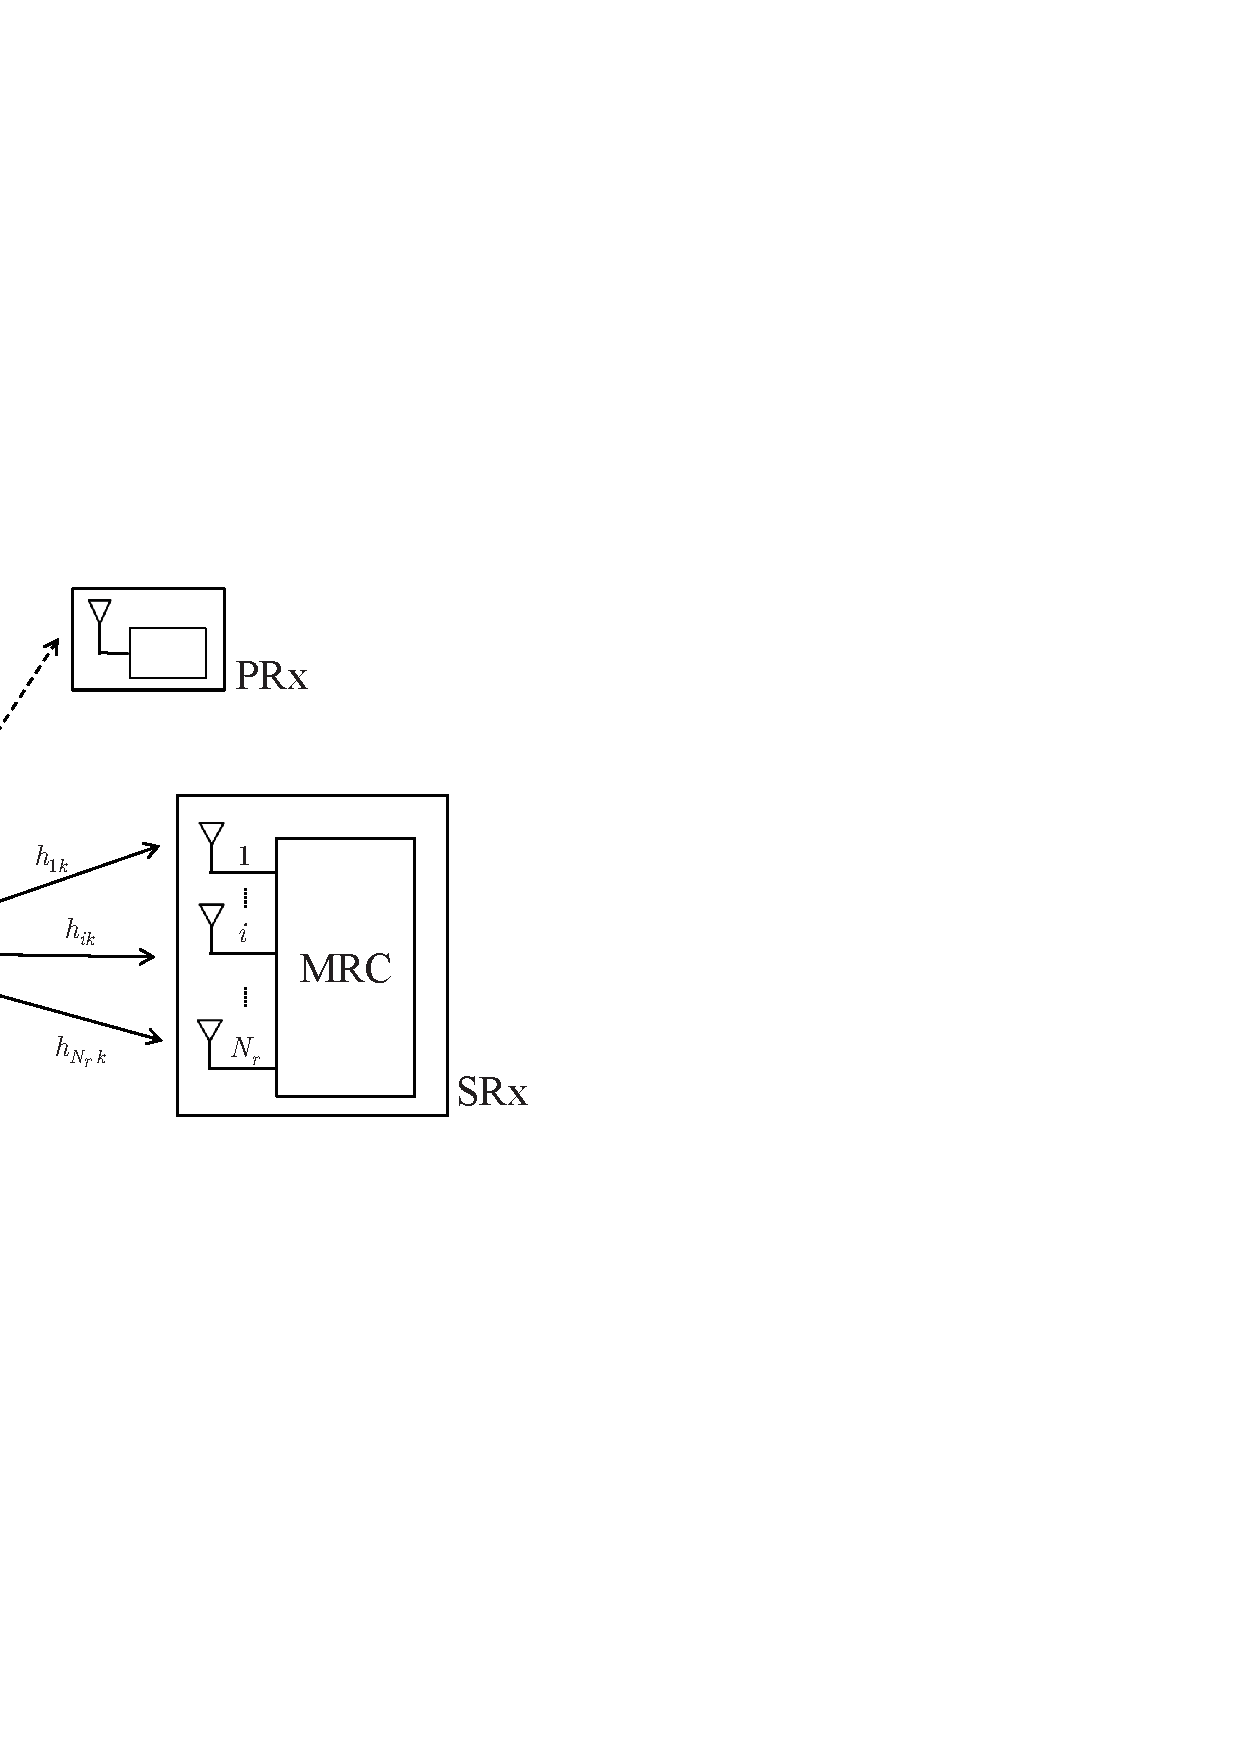
\includegraphics[width=0.75\columnwidth]{plots/model_pdf.pdf}
\caption{System model that consists of an STx with $\Nt$ transmit antennas and one RF chain. It transmits data to an SRx with $\Nr$ antennas and causes interference to the PRx.}
\label{fig:MODEL}
\end{figure}

\newcommand{\hs}{\mathbf{\such}_{s}}
\newcommand{\bhk}[1]{\mathbf{\such}_{#1}}
\newcommand{\hsstar}{\mathbf{\such}_{s^{*}}}
\newcommand{\datasymbol}{d}

\subsection{Antenna Selection Options and Data Transmission}
The STx transmits with power $\Pt$ a data symbol $\datasymbol$, which is drawn with equal probability from a constellation consisting of $M$ symbols. It can select one out of $\Nt$ antennas or it can also decide to transmit with zero power in order to not interfere with the PRx. For ease of exposition, we denote latter option as transmitting from a virtual antenna $\nx$, and define $\hk{1\nx} = 0,\ldots,\hk{\Nr\nx} = 0$, and $\gk{\nx}= 0$. 

Let $s\in\allopts$ denote the antenna selected by the STx. % Thus, STx has $\Nt+1$ options to select from.
 At the $\ith$ receive antenna of the SRx, let $\Rsrx$ denote the signal received and let $\Isrx$ denote the interference from PU transmissions. Let the interference at the PRx due to SU transmissions be $\Iprx$. Then, $\Rsrx$ and $\Iprx$ are given by
%
\begin{align}
\label{eq:r_su}
 \Rsrx &= \sqrt{\Pt}\sqrt{\hk{is}} e^{j\thetahk} \datasymbol + \noise + \Isrx, \\
 \label{eq:i}
 \Iprx &= \sqrt{\Pt}\sqrt{\gk{s}} e^{j\thetagk} \datasymbol ,
\end{align}
%
where $\expect{|\datasymbol|^2}=1$, $\thetahk$ and $\thetagk$ are the phases of the complex baseband STx-SRx and STx-PRx channel gains, respectively, and $\noise$ is a circular symmetric complex additive white Gaussian RV. We assume $\Isrx$ to be Gaussian. Therefore, $\noise + \Isrx\sim \CN\left(\noisevar\right)$. This assumption corresponds to a worst case model for interference at the SRx, and is widely assumed in the literature to ensure tractability~\cite{Sarvendranath_2013_TCOM,Wang_2011_TCom, Kashyap_2014_TCOM,Sarvendranath_2014_TCOM}. It is valid even with one primary transmitter (PTx), if the PTx uses a constant amplitude signal to communicate with the PRx~\cite{Kashyap_2014_TCOM}. With multiple PTxs, it is justified by the central limit theorem. This is also valid when the interference seen at the SRx is negligible, which is assumed in~\cite{musavian_2009_tcom,RZhang_2009_TWC,li_2011_pimrc} and occurs when SRx is located geographically far from the PTx. We refer the reader to~\cite{das_2015_twc} for a comparison of this model with other Gaussian models, such as those that condition on the instantaneous channel power gain of the PTx to SRx link. 

\subsection{CSI Assumptions and Justifications}  
Before we state the optimal TAS rule problem, we discuss the  CSI assumptions below. 
\begin{enumerate}
\item In order to perform TAS, we assume that the STx knows the STx-SRx channel power gains $\Hmx$~\cite{Hanif_2015_globecom,Sarvendranath_2013_TCOM,Wang_2010_TWC,RZhang_2009_TWC,Sarvendranath_2014_TCOM}. However, it need not know the phase information of any of these channels. The SRx uses a coherent demodulator. Hence, it only needs to know the complex channel gains from the selected antenna of the STx to itself, \ie, $\hk{is}$ and $\thetahk$, for $i\in\nropts$. Inserting a pilot symbol along with the data transmitted by the STx can enable this.  

\item We also assume that STx knows the STx-PRx channel power gains $\g$, as has been widely assumed in the underlay CR literature ~\cite{Hanif_2015_globecom,Sarvendranath_2013_TCOM,Sarvendranath_2014_TCOM,Kong_2011_JCN,Wang_2010_TWC,RZhang_2009_TWC}. Different techniques have been studied to estimate  $\g$. These include making the STx sense the primary signal periodically~\cite{Zhao_2008_TSP} or using a power-feedback loop technique~\cite{RZhang_2008_DSAN}. we refer the reader to~\cite{Zhang_2017_tcom} and references there in for a detailed list of methods for obtaining $\g$.  As we shall see, LWIIR  requires the STx to only know if the STx-PRx channel power gain of each antenna exceeds a pre-defined threshold. This is considerably simpler and more robust than accurately estimating $\g$. The SRx does not need to know $\g$. 

\end{enumerate}

\subsection{Problem Statement}
We now formally state our problem. Let $\SEP(\hs)$ denote the instantaneous SEP when antenna $s$ is used for transmission, where $\hs\define\left[\hk{1s},\ldots,\hk{\Nr s} \right]$. From~\cite[(14)]{Chung_2001_TCom}, it is given by  
\begin{equation}
\SEP(\hs) \approx \cone \exp\left({-\frac{\Pt\sumnr\hk{is}}{\ctwo\noisevar} }\right), \quad\text{for} \,\,\, 0\leq s \leq \Nt,
\label{eq:isep}
\end{equation} 
where $\cone$ and $\ctwo$ are modulation-specific constants. The summation term $\sumnr\hk{is}$ in~\eqref{eq:isep} arises because the SRx employs maximal ratio combining (MRC). This formula is exact for differential binary phase-shift-keying (DBPSK) with $(\cone,\ctwo) = (0.5,1)$  and non-coherent binary frequency-shift-keying (NCBFSK) with  $(\cone,\ctwo) = (0.5,2)$~\cite{Fakhan_2014_TSP}. It is very tight approximation with $(\cone,\ctwo )=(0.5,1.7)$ for QPSk,  $(\cone,\ctwo)=(0.6,5.5)$ for 8-PSK, and  $(\cone,\ctwo )=(0.8,8.2)$ for 16-QAM. %It also applies to differential PSK (DPSK) and M-ary frequency-shift-keying (MFSK)~\cite{simon_alouini_book}.


{\em Comments:}
\begin{itemize}
\item While~\eqref{eq:isep} is an approximation for some constellations,  it is accurate, tractable, and applies to a large number of constellations. %We also note that when antenna zero is selected, $\SEP(\hk{\nx})$ tends to  $\cone$,  For the purpose of designing the TAS rule, we will use this formula for all antennas, including $s=\nx$. However, in the average SEP analysis, we will use the accurate value of the SEP defined below for $s=\nx$ as well.
\item Even with zero transmit power ($s=\nx$), the SEP is $\cone<1$, \ie, the SRx can detect correctly with a non-zero probability $1-\cone$. From~\eqref{eq:isep}, the SEP will be less than $1-\cone$ when one of the $1,\ldots,\Nt$ antennas is selected. Therefore, $\cone$ can be interpreted to be a worst case penalty associated with using the zero transmit power option. It ensures that the optimal TAS rule is not trivial, \ie, it does not select $s=\nx$  always in order to cause less interference~\cite{Kashyap_2014_TCOM,Sarvendranath_2013_TCOM,Sarvendranath_2014_TCOM}.\footnote{For a constellation of size $M$, it can be shown that the SEP with zero transmit power is exactly $\zerosep\define 1-\left(1/M\right)$. While we design the TAS rule using~\eqref{eq:isep} for all $\Nt+1$ options in order to ensure tractability, we shall use $\SEP(\h_0) = \zerosep$ in Section~\ref{sec:SEPanalysis} in order to ensure that the SEP analysis is accurate.  } 	
\end{itemize}


{\em TAS Rule Definition:} A TAS rule $\asrule:\brac{\mathbb{R}^{+}}^{\Nr}\times\brac{\mathbb{R}^{+}}^{\Nt} \times \brac{\mathbb{R}^{+}}^{\Nt} \rightarrow \allopts$ is a mapping from $\left(\Hmx,\g\right)$ to the set of $\Nt+1$ available transmit antennas. Thus, $s = \phi(\Hmx,\g)$.

{\em Interference-Outage Constraint:}
From~\eqref{eq:i}, the instantaneous interference power at the PRx is $\Pt\gk{s}$. Therefore, the probability that it exceeds an interference power threshold $\itau$ is equal to $\prob{\Pt\gk{s}>\itau}$. It depends on the TAS rule used through $s$. Since $\Hmx$ and $\g$ are random, so is $s$. Then, the interference-outage constraint can be specified as 
\begin{equation}
\prob{\Pt\gk{s}>\itau} \leq \outmax,
\label{eq:iop_cons}
\end{equation}
where $\outmax$ is the maximum allowed interference-outage probability. 


Let $\asspan$ be the set of all TAS rules. Our goal is to find the optimal TAS rule $\phi^{*}\in\asspan$ that minimizes the average SEP of the secondary system subject to the interference-outage constraint. It can be mathematically stated as the  following stochastic, constrained optimization problem $\optproblem$:
\begin{align}
\label{eq:objective}
\optproblem: \quad \min_{\asrule\,\in\,\asspan} \quad
&\explow{\Hmx,\g}{\SEP(\hs)} \\
\label{eq:cons}
\text{s.t.} \quad &\prob{\Pt\gk{s}>\itau} \leq \outmax, \\
 &s = \phi(\Hmx,\g). 
\end{align}



\section{LWIIR, Its Interference-Outage analysis, and optimality}
\label{sec:analysis}
%
We now propose LWIIR, and characterize its properties and its interference-outage probability. Using these, we prove that LWIIR is indeed the solution of  $\optproblem$ above for a general class of continuous fading models. %We also show that LWIIR and its interference-outage probability expression simplifies as $\lam\tendsto\cone$. 


\subsection{LWIIR and Its Properties}
\label{sec:lambda_rule}
Let 
\begin{equation}
\yk{k} \define \frac{\SEP(\bhk{k})}{\cone} = \exp\left({- \frac{\Pt\sum_{i=1}^{\Nr}\hk{ik}}{\ctwo\noisevar} }\right), \quad \text{for}\,\,  0\leq k \leq\Nt.
\label{eq:yi_def}
\end{equation}
LWIIR is defined in terms of a parameter $\lam \in \left[0, \cone\right]$, and is denoted by $\callamrule$. It is as follows:
\begin{equation}
\callamrule: \quad s=\argmin\limits_{k\in\allopts} \left\{ \ykplusgk{k} \right\}.
\label{eq:lam_weight_rule}
\end{equation}

To understand the behavior of $\callamrule$, we introduce the following terminology. We shall refer to 
%\begin{equation}
$\ykplusgk{k}$
%\label{eq:metric}
%\end{equation}
as the {\em selection metric} of the transmit antenna $k$, for $0\leq k \leq\Nt$. Thus, LWIIR selects the antenna with the smallest selection metric. Further, we shall refer to an antenna $k$ for which $\gklttaubypt{k}$ as an {\em outage-compatible} antenna. Otherwise, we shall refer to it as an {\em outage-incompatible} antenna.  Clearly, antenna zero is always outage-compatible, and its selection metric is $\yk{0}=1$. On the other hand, antenna $k\in\antopts$ can be outage-compatible or outage-incompatible depending on the instantaneous value of $\gk{k}$. We shall also refer to $\lam$ as the {\em interference-outage penalty factor} as it increases the selection metric of, i.e., penalizes, every outage-incompatible antenna. We now characterize  how this selection metric behaves for different values of $\lam$.

\subsubsection{Behavior of LWIIR for Different $\lam$ Values}
\label{sec:LWIIR_prop}
%{\em Behavior of LWIIR for Different $\lam$ Values:}


\begin{enumerate}[a.]
\item For $\lam=0$, the selection metric of antenna $k$ is $\yk{k}$. As $\sumnr\hk{ik}\geq 0$, it follows from~\eqref{eq:yi_def} that $\yk{0}=1\geq\yk{1},\yk{0}\geq\yk{2},\ldots,\yk{0}\geq\yk{\Nt}$, and   $\yk{1},\ldots,\yk{\Nt}$ are monotonically decreasing functions of $\sumnr\hk{i1},\ldots,\sumnr\hk{i\Nt}$, respectively. Hence, 
\begin{equation}
\caluncons:\quad s=\argmin\limits_{k\in\allopts} \left\{ \yk{k} \right\} = \argmin\limits_{k\in\antopts} \left\{ \yk{k} \right\} = \argmax\limits_{k\in\antopts} \left\{\sumnr \hk{ik} \right\}.
\label{eq:uncons_simple}
\end{equation}

From~\eqref{eq:isep}, $\caluncons$ is clearly the optimal TAS rule if the interference-outage constraint in~\eqref{eq:cons} is inactive. We shall, therefore, refer to $\caluncons$ as the {\em interference unconstrained} rule henceforth. Its interference-outage probability $\un$ is given by
%
\begin{equation}
\un= \prob{\gk{s}>\taubypt}= F^c_{\gk{1}}\!\!\left({\taubypt}\right).
\label{eq:uncomsoutage}
\end{equation}
%
The second equality above follows because the antenna $s$ selected by $\caluncons$ does not depend on $\g$, and $\gk{1},\ldots,\gk{\Nt}$ are i.i.d. Thus, $\caluncons$ is the optimal TAS rule when $\outmax \geq \un$. 

\item For $0<\lam<\cone$, the selection metric of antenna $k$ is a linear combination of  an exponentially decreasing function of $\sumnr\hk{ik}$ and $\indic{\gkgrtaubypt{k}}$, which is a discontinuous function of $\gk{k}$. A three-dimensional view of this selection metric as a function of $\sumnr\hk{ik}$ and $\gk{k}$ is shown in Figure~\ref{fig:metric}. Notice its discontinuous behavior, which happens at $\gk{k}=\taubypt$. It is different from the TAS rules proposed for other interference constraints~\cite{Fakhan_2014_TSP,Wang_2010_TWC,Wang_2011_TCom,Sarvendranath_2013_TCOM,Sarvendranath_2014_TCOM}.

\item For $\lam=\cone$, the selection metric of any outage-incompatible antenna $k$ is  $\yk{k}+1\geq 1$. It exceeds the selection metric of antenna zero. Therefore, LWIIR will select an antenna with the largest $\sumnr\hk{ik}$ only from the set of outage-compatible antennas. Only for this special case, it is equivalent to the TAS rule in~\cite{Hanif_2015_globecom}  for the peak interference constraint.

%\item A necessary but not sufficient condition for virtual antenna zero to be selected is that all the $\Nt$ antennas $1,\ldots,\Nt$ are outage-incompatible. This is because the selection metric of any outage-compatible antenna $i$, for $1\le i \leq \Nt$, is less than that of antenna zero, \ie, $\yk{i}<\yk{0}$.

\end{enumerate}

\begin{figure}
\centering 
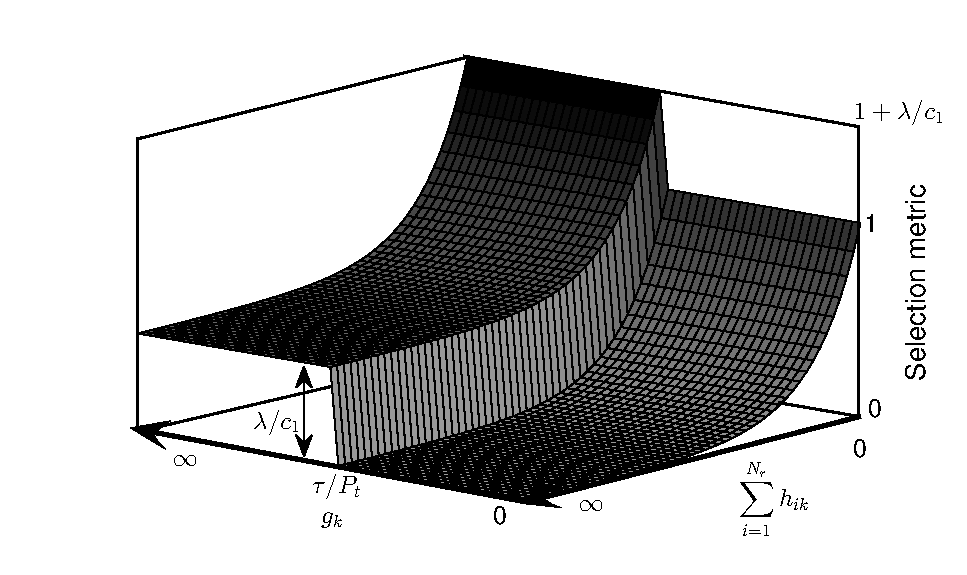
\includegraphics[width=\linewidth]{plots/selection_metric_3d.eps}
\caption{Selection metric of antenna $k$ as a function of $\sumnr\hk{ik}$ and $\gk{k}$.}
\label{fig:metric}
\end{figure}

\subsection{Interference-Outage Probability and Optimality of LWIIR}
We first derive the interference-outage probability of LWIIR in terms of the probability distribution of $\yk{1},\ldots,\yk{\Nt}$. Since $\yk{1},\ldots,\yk{\Nt}$ are identically distributed, we denote their marginal CCDF and PDF by $F_{y}^{c}(\cdot)$ and $f_{y}(\cdot)$, respectively. 
\begin{lemma}
\label{lem:outage_Nt}
The interference-outage probability $\outlam$ of LWIIR, for $0\leq\lam\leq\cone$, is given by
\begin{equation}
\label{eq:pr_outage_ccdf} 
\outlam  =  \Nt\un \int_{0}^{1-\lambym} 	
\left[ \un F_{y}^{c}\left(x\right) + \left(1 -\un\right)F_{y}^{c}\left(x+\lambym\right) \right]^{\Nt-1} f_{y}(x)\,dx.
\end{equation}
For the class of continuous fading models, $\outlam$ is a continuous and strictly monotonically decreasing function of $\lam$. Furthermore, for any $\outmax\in[0,\un]$, a unique $\lam\in[0,\cone]$ exists such that $\outlam=\outmax$. 
\end{lemma}
%
\begin{IEEEproof}
    The proof is given in Appendix~\ref{proof:outage_Nt}.
\end{IEEEproof}
%
%Note that~\eqref{eq:pr_outage_ccdf} reduces to $\un$ when $\lam=0$, which corresponds to the interference unconstrained rule. Further, $\outlam=0$ when $\lam=\cone$, which corresponds to the peak interference constrained rule.  

{\em Insights:} Replacing $x+\lambym$ with $\lambym$ in~\eqref{eq:pr_outage_ccdf}, the following closed-form bound for $\outlam$ follows: 
%
\begin{equation}
\label{eq:pr_outage_ub}
\outlam  \leq \left[ \un + \left(1-\un\right)F_{y}^{c}\left(\lambym\right)  \right]^{\Nt} - \left[ \un F_{y}^{c}\left(1-\lambym\right) + \left(1-\un\right)F_{y}^{c}\left(\lambym\right)  \right]^{\Nt}.
\end{equation}
%
In Section~\ref{sec:results}, we shall see that this upper bound is tight. For $\Nt = 2$, the following different, simpler bound can also be derived: 
%
\begin{equation}
\label{eq:two_Nt_UB}
\outlam \leq \un^2 + 2\un(1-\un)F_{y}^{c}\left(\lambym\right).
\end{equation}
For example, for Rayleigh fading and $\Nr=1$, equating~\eqref{eq:two_Nt_UB} to $\outmax$ yields the following closed-form upper bound for $\lam$. It holds for $\itau\geq-\left( \Pt\mug/{2}\right) \ln\left({\outmax}\right)$.
%
\begin{equation}
\label{eq:two_Nt_lam}
\lam \leq \cone \left( \frac{2\un - \un^2 - \outmax}{2\un(1-\un)} \right)^{\snrbyal[]}.
\end{equation} 


Using Lemma~\ref{lem:outage_Nt}, we prove the following result. 
%
\begin{result}
\label{thm:selection_rule_on_off}
The optimal TAS rule that solves $\optproblem$ lies in the set of rules $\set{\callamrule:0\leq\lam\leq\cone}$. If $\outmax\geq\un$, then it is given by $\caluncons$. Else, for $0\leq\outmax<\un$, it is given by $\callamstarrule$, where $\lamstar>0$  is the solution of $\outlam=\outmax$. Such a choice of $\lamstar$ is unique, strictly positive, and always exists. 
\end{result}
%                
\begin{IEEEproof}
   The proof is given in Appendix~\ref{proof:selection_rule_on_off}.
\end{IEEEproof}
%

Notice that $\callamrule$ only needs to know whether or not the STx-PRx channel power gains $\g$ exceed a threshold $\tau/\Pt$ and not their exact values. This makes it robust to errors in estimating $\g$. 

\subsection{Insights: A Simpler, Intuitive  TAS Rule and Its Interference-Outage Probability}
In this section, we gain new insights about LWIIR when $\lam \tendsto \cone$. This happens when the probability that the antennas $1,\ldots,\Nt$ are all outage-incompatible exceeds $\outmax$, \ie, $\un^{\Nt}>\outmax$.    %$\prob{\gkgrtaubypt{1}}^{\Nt}>\outmax$.   
%

\newcommand{\gammath}{\eta}
For a given realization of the channel gains, let $\goodset$ denote the set of all outage-compatible antennas. First, consider the case when $\goodset\neq\nullset$. From Comment c in Section~\ref{sec:LWIIR_prop}, it follows that as $\lam \tendsto \cone$, $\callamrule$ becomes 
\begin{equation}
\label{eq:hp_rule_G_not_empty}
s = \argmax_{k\in\goodset}\left\lbrace \sumnr \hk{ik}\right\rbrace. 
\end{equation}
Now, consider the case when $\goodset= \nullset$. As all the antennas are outage-incompatible, $\callamrule$ becomes $s = \argmin\left\lbrace  \yk{0},\yk{1}+\lambym,\ldots,\yk{\Nt}+\lambym \right\rbrace$. Using $\yk{0}=1$ and \eqref{eq:yi_def}, the selection rule for this case can be shown to simplify to  
\begin{equation}
\label{eq:hp_rule_G_empty}
s = \left\{
\begin{array}{ll}
0 , & \text{if}~\sumnr\hk{i1}\leq\gammath,\ldots, \sumnr\hk{i\Nt}\leq\gammath, \\
\argmax\limits_{k\in\antopts}\left\lbrace \sumnr\hk{ik}\right\rbrace , &\text{otherwise},
\end{array}\right.
\end{equation}
where $\gammath\define\igammainline$. Hence, $\callamrule$ selects antenna $s\neq0$ if and only if there is at least one antenna $k\in\antopts$ for which $\sumnr \hk{ik}$ exceeds $\gammath$. Else, $s=0$. 


{\em Interference-Outage Probability:} For the above TAS rule in~\eqref{eq:hp_rule_G_empty} , interference-outage happens only when $\goodset=\nullset$ and  $s\neq\nx$. Hence,  $\outlam=\prob{{\goodset}=\nullset, s \neq 0}$. This can be shown to be equal to
\begin{equation}
\label{eq:pr_outage_hp}
\outlam = \un^{\Nt} - \un^{\Nt}\left(\ccdfyrv{1-\lambym} \right)^{\Nt}.
%\outlam  =  \un^{\Nt} - \un^{\Nt}\left[1 - \left(1-\lambym\right)^{\albysnr[]} \right]^{\Nt}.
\end{equation}
%
%Alternatively,~\eqref{eq:pr_outage_hp} is the asymptotic expression for the interference-outage probability as $\lam\tendsto\cone$.
For Rayleigh fading and $\Nr=1$, equating~\eqref{eq:pr_outage_hp} with $\outmax$ yields the following closed-form expression for $\lam$ for $\itau<-\left({\Pt\mug}/{\Nt}\right) \ln\left({\outmax}\right)$: 
\begin{equation}
\label{eq:lam_asym}
\lam  =  \cone - \cone\left(1 - \left[1 - \frac{\outmax}{\un^{\Nt}}\right]^{\frac{1}{\Nt}} \right)^{\snrbyal[]}.
\end{equation}
%


%Note that the above upper bound will be less than or equal to $\cone$ only when $\frac{2\un - \un^2 - \outmax}{2\un(1-\un)}\leq 1$, which simplifies to $\un^2 \leq \outmax$, which is equivalent to $\itau\geq\left({\Pt\mug}/{2}\right)\ln\left(1/\outmax\right)$.
%which means for $\Pt<\frac{2\tau}{\mug\ln\left(1/\outmax\right)}$. 


\section{SEP Analysis of LWIIR}
\label{sec:SEPanalysis}
Having proved that LWIIR is SEP-optimal, we derive an expression for its average SEP, which we denote by  $\avgSEP$. We do this for the general case of $\Nt$ transmit antennas and $\Nr$ receive antennas for any continuous fading model. It turns out to be in a single integral form that depends on the CCDF $\ccdfyrv{\cdot}$ and PDF $\pdfy{\cdot}$. It can be expressed as an integral-free summation using Gaussian integration of moments~\cite[pp 921-922]{abramowitz_stegun}. We also study an insightful case for which the $\avgSEP$ simplifies to a closed form. %We conclude this section with asymptotic behavior of LWIIR as $\lam\tendsto\cone$. 
 
%In this section, we derive the average SEP expression for an interference-outage constrained underlay CR when LWIIR is employed. First, we do this for a secondary system with $\Nt$ transmit antennas and $\Nr$ receive antennas for any continuous fading model. Then, we show that this average SEP expression can be simplified to a closed-form for Rayleigh fading when $\Nr=1$.

\begin{result}
\label{thm:SEP_exact_Nt_gen}
$\avgSEP$ of $\callamrule$ for a continuous fading model is given by
\begin{equation}
\label{eq:SEP_Nt_gen} 
\avgSEP= \zerosep\left[\unccdfygen{\un}{1-\lambym}\right]^{\Nt} + \termtwo,
\end{equation}
%
where $\zerosep=1-\frac{1}{M}$ and
\begin{multline}
\hspace{25pt}\termtwo \!= \Nt\cone(1-\un)\int_{0}^{\lambym} \left[\un + \unccdfygen{(1-\un)}{x}\right]^{\Nt-1} x\pdfyNrgen{x} dx\\
\hspace{-30pt}+ \Nt\cone \int_{0}^{1-\lambym}
\left[\unccdfygen{\un}{x} +\unccdfygen{(1-\un)}{x+\lambym}  \right]^{\Nt-1}\\
\times\left(\un x\pdfyNrgen{x} + (1-\un)\left(x + \lambym\right) \pdfyNrgen{x + \lambym}\right) dx.
\label{eq:termtwo_gen}
\end{multline}
%
\end{result}
%
\begin{IEEEproof}
The proof is given in Appendix~\ref{proof:SEP_exact_Nt_gen}.
\end{IEEEproof}
%

The first term in~\eqref{eq:SEP_Nt_gen} corresponds to the average SEP due to $s=\nx$. It increases as the interference-outage penalty factor $\lam$ increases. This is because a higher $\lam$ corresponds to a tighter interference-outage constraint, which increases the probability of selecting $s=\nx$. 
%
%\begin{multline}\label{eq:SEP_Nt_Nr_rayleigh} \frac{\Nt\cone(1-\un)}{\Gamma(Nr)}\left(\albysnr\right)^{Nr}\int_{0}^{\lambym} \left(\un + \unccdfy{(1-\un)}{x}\right)^{\Nt-1} \ytimespdfyNr dx\\ + \frac{\Nt\cone}{\Gamma(Nr)}\left(\albysnr\right)^{Nr} \int_{0}^{1-\lambym} \left(\unccdfy{(1-\un)}{\left(x+\lambym\right)} + \unccdfy{\un}{x}\right)^{\Nt-1}\\ \times\left((1-\un)\ypluslamtimespdfyNr+\un\ytimespdfyNr\right) dx\\ +\zerosep\left(\unccdfy{\un}{\left(1-\lambym\right)}\right)^{\Nt}.                                     \end{multline}

For Rayleigh fading, in which $\hk{ik}$ and $\gk{k}$ are i.i.d.\ exponential RVs with means $\muh$ and $\mug$, respectively, it can be shown that the unconstrained interference-outage probability $\un$ is equal to $\inlccdfg[]$. Thus, LWIIR is the same as the interference unconstrained rule $\caluncons$ for $\itau\geq-\Pt\mug\ln\left(\outmax\right)$.  Let $\snr\define\Pt\muh/\noisevar$ denote the mean signal-to-noise-ratio (SNR) of the SU. Thus, the CCDF and PDF of the RV $\yk{1}$ are given by 
\begin{align}
\label{eq:ccdfyNr}
\ccdfyrv{x} &= \ccdfyNr{x}, \quad \text{for}\,\, x \in (0,1],\\
\label{eq:pdfyNr}
\pdfyNrgen{x} &= \pdfyNr, \quad \text{for}\,\,  x \in (0,1],
\end{align}
where $\gamma(\cdot,\cdot)$ denotes the lower incomplete gamma function~\cite[(8.350.1)]{gradshteyn00_book}. Note that further simplification of~\eqref{eq:termtwo_gen} is not possible even for the special case due to the lower incomplete gamma function inside the integral.  
%
\subsection{Special Case: Rayleigh Fading and $\Nr=1$} 
For $\Nr=1$,~\eqref{eq:ccdfyNr} and~\eqref{eq:pdfyNr} simplify to $F_{y}^{c}(x) = 1-x^{\albysnr}$ and $f_{y}(x) = \al x^{\albysnr-1}/\snr$, for $x \in (0,1]$. Upon substituting these in~\eqref{eq:SEP_Nt_gen}, $\avgSEP$ simplifies to 
%
\newcommand{\lidx}{l}
\newcommand{\midx}{m}
\begin{multline}
\label{eq:avgSEPoneNr} 
\avgSEP =\zerosep\un^{\Nt}\!\left[1-\left(1-\lambym\right)^{\!\albysnr[]}\right]^{\Nt}
+ \frac{\Nt\un^{\Nt}\al\lam}{\snr} \sum_{k=0}^{\Nt-1}\sum_{\lidx=0}^{k} \frac{\nck{\Nt-1}{k} \nck{k}{\lidx}\left(\lambym\right)^{\albysnr[(\lidx+1)]}\left(1-\un\right)^{k+1} }{(-1)^{\lidx} \left( \albysnr[(\lidx+1)]+1\right)\un^{k+1} }\\ + \frac{\Nt\cone\al}{\snr} \sum_{k=0}^{\Nt-1} \sum_{\lidx=0}^{k} \sum_{\midx=0}^{\Nt-k-1} (-1)^{\lidx+\midx}  \binom{\Nt-1}{k} \binom{k}{\lidx} \binom{\Nt-k-1}{\midx} \\\times\un^{k} (1-\un)^{\Nt-k-1} \left[ \un\psifun{\midx}{\lidx+1} +  \left(1-\un\right) \psifun{\midx+1}{\lidx} \right]
,
\end{multline}
where $\psifun{k_1}{k_2} = \int_{0}^{1-\frac{\lam}{\cone}} \left(x+\lambym\right)^{\albysnr[k_1]} x^{\albysnr[k_2]} \,dx$.
%
\newcommand{\gqsym}{z_{\lidx}}
\newcommand{\gqwt}{w_{\lidx}}
In general, $\psifun{k_1}{k_2}$ can be computed accurately as a sum of $n$  terms as follows: 
\begin{equation}
\psifun{k_1}{k_2} ={\onemlc^{\albysnr[k_2]+1}} \sum_{\lidx=1}^{n} \gqwt {\left(\!\gqsym\onemlc +\lambym\right)}^{\albysnr[k_1]} \gqsym^{\albysnr[k_2]} + \error,
\label{eq:gauss_quad}
\end{equation}
where $\gqsym$ and $\gqwt$ are the $n$ abscissas and weights for Gaussian integration of moments~\cite[pp 921-922]{abramowitz_stegun}, respectively. The error term $\error$ decreases as $O(1/n^2)$~\cite{Xiang_2012_SIAM}, where $O(\cdot)$ is as per the Bachmann-Landau notation~\cite[Chap. 3]{CLRS_algo_book}. In Section~\ref{sec:results}, we will see that~\eqref{eq:gauss_quad}  is accurate even for $n$ as small as 4. Furthermore, for $\lam\in({\cone}/{2}, \cone]$, $\psifun{k_1}{k_2}$ can be written explicitly as the following infinite series~\cite{gradshteyn00_book}:
%
%\begin{multline}
%\psifun{k_1}{k_2} = \frac{\left(\lambym\right)^{\albysnr[k_1]} \left(1-\lambym\right)^{\albysnr[k_2]+1}}{\albysnr[k_2]+1} \\
%+ \sum_{\midx=1}^{\infty}\! \frac{\akone\!\!\left(\akone\!-\!1\right)\!\ldots\!\left(\akone\!-\!\midx\!+\!1\right)\!\left(\!\lambym\!\right)^{\!\!\albysnr[k_1]  - \midx} \!\!\left(\!1\!-\!\lambym\!\right)^{\!\!\albysnr[k_2]+\midx+1}}{\midx ! \left(\albysnr[k_2]+\midx+1\right)}. 
%\label{eq:inf_sum}
%\end{multline}
%
\begin{equation}
\psifun{k_1}{k_2} = \sum_{\midx=0}^{\infty} \frac{\Gamma\left(\akone+1 \right) \left(\lambym\right)^{\albysnr[k_1]  - \midx} \left(1-\lambym\right)^{\albysnr[k_2]+\midx+1}}{\Gamma\left(\akone-\midx+1 \right)\midx ! \left(\albysnr[k_2]+\midx+1\right)}. 
\label{eq:inf_sum}
\end{equation}
Four terms in the above summation turn out to be sufficient to accurately compute~\eqref{eq:inf_sum}.  
%
%Using Gauss quadrature~\cite{abramowitz_stegun}, 
%


\section{Impact of Imperfect CSI on LWIIR}
\label{sec:imperfectcsi}
We now study the behavior of LWIIR when the STx has imperfect estimates of the STx-SRx and STx-PRx channel power gains for Rayleigh fading, as is the case in practice. For tractability, we assume that the SRx knows perfectly the $\Nr$ complex channel gains corresponding to the transmit antenna selected. %We derive the analytical expressions for the interference-outage probability at the PRx and the average SEP of the SU with imperfect CSI. 


{\em Channel Estimation Model}: We consider minimum mean square error (MMSE) channel estimation model~\cite{Sboui_2013_TWC,Kashyap_2014_TCOM,musavian_2009_tcom}. We refer reader to~\cite{Zhang_2017_tcom,Kashyap_2015_wicomlet} and references there in for comparison of different channel estimation models.  Let $ \sugain{ik}= \sqrt{\hk{ik}}e^{-j\suchph_{ik}}\sim\CN\left(\muh\right) $ denote the complex baseband channel gain of the link from $\kth$ transmit antenna of the STx to the $\ith$ receive antenna of the SRx, and let $\pugain{k} = \sqrt{\gk{k}}e^{-j\puchph_{k}}\sim\CN\left(\mug\right)$ denote the complex baseband channel gain from the $\kth$ antenna of the STx to the PRx. Let $\sugainhat{ik}$ and $\pugainhat{k}$ denote the MMSE estimates of $\sugain{ik}$ and $\pugain{k}$, which are based on pilot transmissions by SRx and PRx with powers $\hpilotpower$ and $\gpilotpower$, respectively.  It can be shown that  $\sugainhat{ik}\sim\CN\left(\muhhat \right)$ and $\pugainhat{k}\sim \CN\left(\mughat\right)$, where  $\muhhat ={\hpilotpower\mu^2_{\such}}/{\left( \hpilotpower\muh+1\right)}$ and $\mughat = {\gpilotpower\mu^2_{\puch}}/{\left( \gpilotpower\mug+1\right)}$~\cite{Kashyap_2014_TCOM}.  
This implies that the channel power gain estimates $\hkhat{ik}=|\sugainhat{ik}|^2$ and $\gkhat{k}=|\pugainhat{k}|^2$ are i.i.d. exponential RVs with means $\muhhat$ and $\mughat$, respectively. Furthermore, the correlation coefficient  of the RVs $\hk{ik}$ and $\hkhat{ik}$ is $\rhoh\define{\hpilotpower\muh}/{\left( \hpilotpower\muh + 1\right) }$, and that of $\gk{k}$ and $\gkhat{k}$ is $\rhog \define{\gpilotpower\mug}/{\left( \gpilotpower\mug + 1\right) }$. 

Since the STx knows $\hkhat{ik}$ and $\gkhat{k}$, it selects its transmit antenna as follows: 
\begin{equation}
\callamrule:\quad s=\argmin\limits_{k\in\allopts} \left\{ \ykhatplusgkhat{k} \right\},
\label{eq:shat}
\end{equation}
%Recall that $\lamstar$ is obtained by equating interference-outage probability $\outlam$ with perfect CSI in~\eqref{eq:pr_outage_ccdf} to $\outmax$. 
where 
\begin{equation}
\ykhat{k} \define  \exp\left({- \frac{\Pt\sum_{i=1}^{\Nr}\hkhat{ik}}{\ctwo\noisevar} }\right), \quad \text{for} \quad 0\leq k \leq\Nt,
\label{eq:yihat_def}
\end{equation}
$\hkhat{1\nx} \define 0,\ldots,\hkhat{\Nr\nx} \define 0$, and $\gkhat{\nx} \define 0$. Let $F_{\yhat}^{c}(\cdot)$ and $f_{\yhat}(\cdot)$ denote the CCDF and PDF, respectively, of the i.i.d. RVs $\ykhat{1},\dots,\ykhat{\Nt}$. They are given by $F_{\yhat}^{c}\left(x\right) =  {\gamma\left(\Nr,-\ctwo\ln(x)/\snrhat\right)} \left/ {(\Nr-1)!}\right.$ and $f_{\yhat}\left(x\right) = { \left( \ctwo/\snrhat \right)^{\Nr} \left(-\ln\left(x \right)\right)^{\Nr-1} x^{\left( \ctwo/\snrhat \right) - 1}}\left/{(\Nr-1)!}\right.$, for $x \in (0,1]$.  Let  $\unhat\define\ccdfghatinline$ and  $\snrhat\define{\Pt\muhhat}/{\noisevar}$.  


\newcommand{\D}{\Delta}

\newcommand{\pdfyhatNr}{\left(\ln\left(\frac{1}{x}\right)\right)^{\Nr-1}x^{\albysnr[]-1}} % only y terms constants taken care separately
\newcommand{\yhattimespdfyNr}{\left[-\ln\left(x\right)\right]^{\Nr-1}x^{\D}} % only y terms constants taken care separately
\newcommand{\yhatpluslamstartimespdfyNr}{\left[-\ln\left({x+\lamstarbym}\right)\right]^{\Nr-1}\left(x+\lamstarbym\right)^{\D}} % only y terms constants taken care separately
\newcommand{\yhatpluslamtimespdfyNr}{\left[-\ln\left({x+\lambym}\right)\right]^{\Nr-1}\left(x+\lambym\right)^{\!\!\D}} % only y terms constants taken care separately
\newcommand{\unccdfyhat}[2]{{#1}\,\,\ccdfyhatrv{#2}}


\newcommand{\avgSEPhat}{\widehat{\SEP}}

\subsubsection{ Average SEP} The average SEP of the above TAS rule is given as follows. 

\begin{result}
\label{thm:avg_SEP_imperfect}
$\avgSEP$ of $\callamrule$ for an $\Nt\times\Nr$ CR system with imperfect CSI at the STx is given by
\begin{multline}
\label{eq:avg_SEP_imperfect}
\avgSEP = \frac{\Nt \T^{\Nr}\cone(1-\unhat)}{(\Nr-1)!} \int_{0}^{\lambym} \left[\unhat + \unccdfyhat{(1-\unhat)}{x}\right]^{\Nt-1} \yhattimespdfyNr\, dx\\
\hspace{60pt} + \frac{\Nt \T^{\Nr}\cone}{(\Nr-1)!} \int_{0}^{1-\lambym}
\!\left[\unccdfyhat{\unhat}{x} + \unccdfyhat{(1-\unhat)}{x+\lambym} \right]^{\Nt-1} \!\!\Bigg(\unhat\yhattimespdfyNr  \\ 
\hspace{40pt}\left. + (1-\unhat)\yhatpluslamtimespdfyNr\right)\, dx 
+\zerosep\left[\unccdfyhat{\unhat}{1-\lambym}\right]^{\Nt}\!\!,\!\!
\end{multline}
where $\T \define \Tc$ and $\D \define \Dc$.	
\end{result}
\begin{IEEEproof}
	The proof is given in Appendix~\ref{proof:avg_SEP_imperfect_CSI}.
\end{IEEEproof}

%Substituting $\snrhat=\snr$, $\rhoh=1$, and $\unhat=\un$ in~\eqref{eq:avg_SEP_imperfect} reduces it to the average SEP expression for the perfect CSI case in~\eqref{eq:SEP_Nt_gen}. 
Further simplification of $\avgSEP$ in~\eqref{eq:avg_SEP_imperfect} is not possible due to the involved form of the integrand. However, for $\Nr=1$, simplified expressions can be obtained along lines similar to that for the perfect CSI case in~\eqref{eq:avgSEPoneNr}. These are not shown here to conserve space.



\subsubsection{ Interference-Outage Probability} We now derive the interference-outage probability for the TAS rule in~\eqref{eq:shat}.

\begin{result}
\label{thm:outage_imperfect_CSI}
  The interference-outage probability $\outlam$ of $\callamrule$ with imperfect CSI is given by
\begin{multline}
\label{eq:pr_outage_impefect} 
\!\outlam \!=\! \Nt \!\int_{0}^{1-\lambym} 	
\!\left[ \unhat F_{\yhat}^{c}\left(x\right) + \left(1 -\unhat\right)F_{\yhat}^{c}\left(x+\lambym\right)\right]^{\Nt-1}\!\! \left(\! (\un - \Probglt) f_{\yhat}\left(x\right)  \!+\!  \Probglt f_{\yhat}\!\left(\! x+\lambym\right) \!\right)\, dx\\
+ \frac{ \Probglt}{1 - \unhat} \left( 1 - \left[\unhat + \left(1 -\unhat\right)F_{\yhat}^{c}\left(\lambym\right)  \right]^{\Nt}  \right),
\end{multline}
%
%\begin{multline}
%\label{eq:pr_outage_imperfect_ub}
%\outlam  \leq \frac{\un - \Probglt}{\unhat}\left( \left[\unhat + \left(1-\unhat\right)F_{\yhat}^{c}\left(\lambym\right)\right]^{\Nt} - \left[ \unhat F_{\yhat}^{c}\left(1-\lambym\right) + \left(1-\unhat\right)F_{\yhat}^{c}\left(\lambym\right)\right]^{\Nt}\right) \\+  \frac{ \Probglt \left( 1-\unhat^{\Nt}\right) }{1-\unhat},
%\end{multline}
%
%respectively,
where  $\Probglt \!=\! \un  Q_1\!\left(\frac{\rhog}{ \gpilotpower} \sqrt{\frac{2\itau}{ \gpilotpower\Pt}},\sqrt{\frac{2 \gpilotpower\itau}{\Pt}}\right) \! - \frac{\unhat}{2} \left(\! 1 + e^{-\frac{2\itau\rhog}{ \gpilotpower\Pt}}I_{0}\!\left(\frac{2\itau\rhog}{ \gpilotpower\Pt} \right) \!\right)$, $I_{0}(\cdot)$ is the modified Bessel function of zeroth order~\cite[(8.406.3)]{gradshteyn00_book}, and  $Q_1(\cdot,\cdot)$ is the Marcum-Q function~\cite[(4.34)]{simon_alouini_book}.  %,  and $f_{\yhat}\left( x\right) = \frac{ \left( \albysnrhat \right)^{\Nr} \left(-\ln\left(x \right)\right)^{\Nr-1} x^{\albysnrhat - 1}}{(\Nr-1)!}$.
\end{result}
%
\begin{IEEEproof}
	The proof is given in Appendix~\ref{proof:outage_imperfect_CSI}.
\end{IEEEproof}
%

Note: In the interference-outage unconstrained case $\left(\lam=0\right)$, $\outlam$ in~\eqref{eq:pr_outage_impefect} reduces to $\un$ even for the imperfect CSI. This is because when $\lam=0$, the selected  antenna does not depend on the  STx-PRx channel power gain estimates. Furthermore, in the peak interference power constrained case $\left(\lam=\cone\right)$, it simplifies to $\frac{ \Probglt \left( 1-\unhat^{\Nt}\right) }{1-\unhat}$, while it is zero for perfect CSI. Similar to~\eqref{eq:pr_outage_ub}, we can derive a closed-form upper bound for $\outlam$ in~\eqref{eq:pr_outage_impefect} as well.





\section{Numerical Results and Performance Benchmarking}
\label{sec:results}
We now present Monte Carlo simulations that measure the average SEP over  $10^6$ data symbol transmissions to verify our analytical results and quantify the behavior of LWIIR as a function of different system parameters. These simulate the entire transmit and receive chains and do not assume the formula in~\eqref{eq:isep}. We also benchmark its performance against other TAS rules proposed in the literature and study the impact of imperfect CSI. We shall set $\lam$ to be optimal interference-outage penalty factor $\lamstar$ for which $\outlam= \outmax$, for $0 \leq \outmax < \un$ and $\lam=0$,  for $\outmax \geq \un$. We set $\noisevar =1$ and $\muh =\mug = 1$, and show results for Rayleigh fading. 

Figure~\ref{fig:SEP_vs_tau} plots the average SEP of LWIIR as a function of the interference power threshold $\itau$ for different numbers of transmit and receive antennas. Analytical results using~\eqref{eq:SEP_Nt_gen} are also shown. They match well with the simulations. The average SEP behavior depends on which of the two regions the interference power threshold $\itau$ lies. (i) {\em Interference-outage constrained region $(\itau < 8.6$~dB):} In this region, the interference-outage constraint in~\eqref{eq:cons} is active ($\lam>0$). In general, this happens for $\itau\!<\!-\Pt\mug\ln\left(\outmax\right)$; it is independent of $\Nt$ and $\Nr$. Here, the average SEP decreases as $\itau$ increases because the interference power allowed at the PRx increases. (ii) {\em Interference-outage unconstrained region $(\itau \geq 8.6$~dB):} In this region, the interference-outage constraint is inactive ($\lam=0$). Here, the average SEP decreases to a constant value as LWIIR is same as the interference unconstrained rule $\caluncons$. This constant decreases exponentially as $\Nt$ or $\Nr$ increase due to more spatial diversity. Also plotted is the average SEP of LWIIR when $\lam$ is obtained by equating the integral-free upper bound for $\outlam$ in~\eqref{eq:pr_outage_ub} to $\outmax$. We see that the degradation in the average SEP  is negligible when compared to using the exact $\lam$ that is computed from the more involved equation in~\eqref{eq:pr_outage_ccdf}. 

\begin{figure}
  \centering 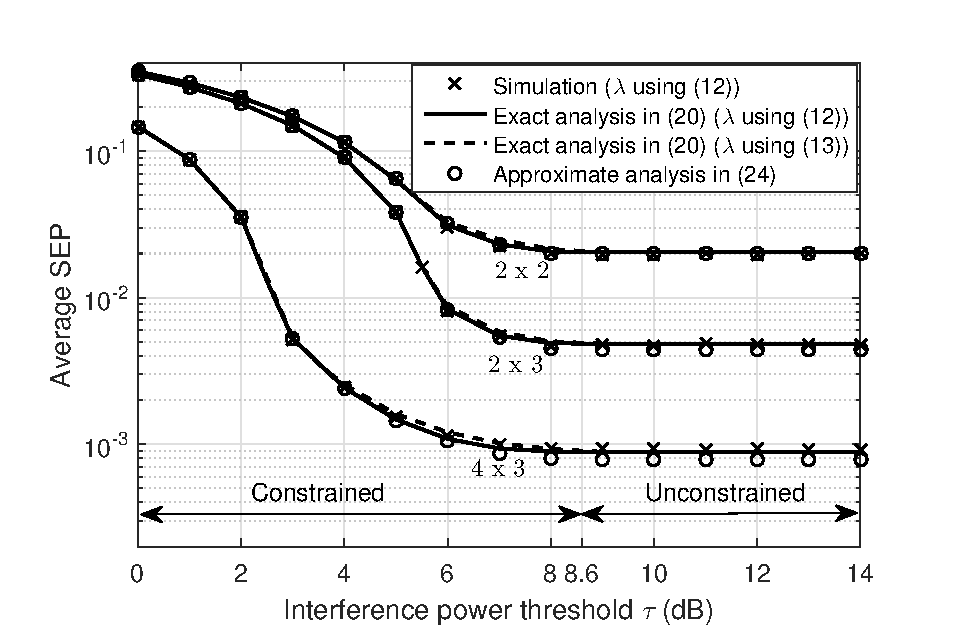
\includegraphics[width=\linewidth]{plots/PCSI_SEP_vs_tau_pout_10_PT_5dB_Nt_2_4_Nr_2_3_M_4.eps}
  \caption{Average SEP as a function of interference power threshold $\itau$ for different $\Nt \times \Nr$ values ($\outmax=0.1$,  $\Pt = 5$~dB, and QPSK).}
\label{fig:SEP_vs_tau}
\end{figure}

Figure~\ref{fig:SEP_vs_tau_QAM} plots the average SEP as a function of interference power threshold $\tau$. This is done for 8-PSK and 16-QAM, and for two values of $\outmax$. The simplified average SEP formula for $\Nr=1$ in~\eqref{eq:avgSEPoneNr} and its approximation in~\eqref{eq:gauss_quad} with $n = 4$ terms for 16-QAM and $n=8$ terms for 8-PSK  are plotted. We observe that both~\eqref{eq:avgSEPoneNr} and~\eqref{eq:gauss_quad} match well with simulations. In the interference-outage constrained region, the average SEP decreases as $\outmax$ increases as the interference constraint becomes more relaxed. In the interference-outage unconstrained region, the average SEP reaches a floor that is  independent of $\outmax$.  %This boundary value is independent of the  constellations size and is equal to $16.6$~dB when $\outmax=0.1$. 

\begin{figure}
	\centering 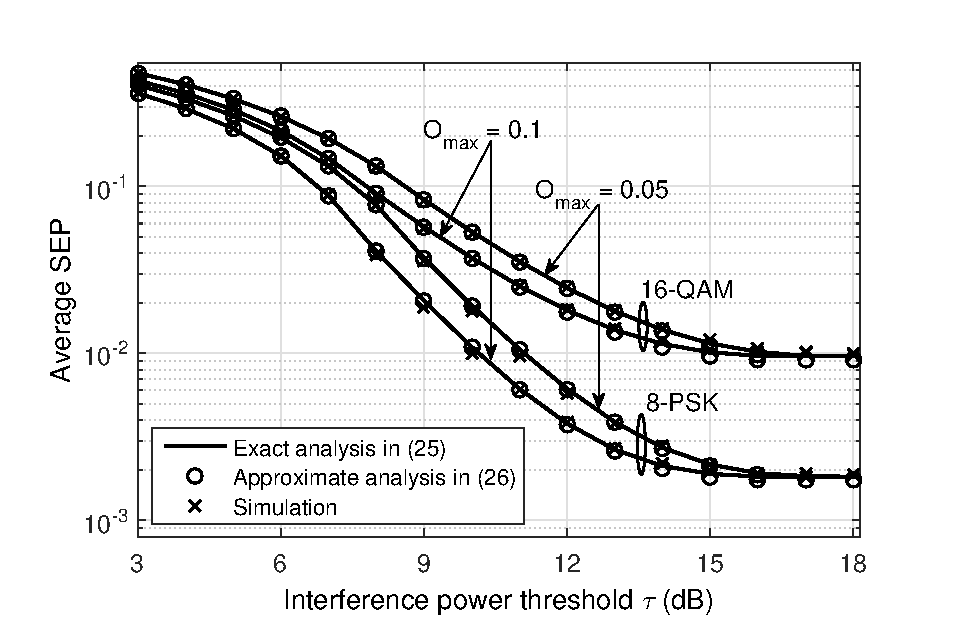
\includegraphics[width=\linewidth]{plots/CURVE_FIT_SEP_vs_tau_pout_5_10_PT_13dB_Nt_8_M_8_16.eps}
	\caption{Average SEP as a function of interference power threshold $\itau$ for 8-PSK and 16-QAM for different values of $\outmax$ ($\Pt = 13$~dB, $\Nt=8$, and $\Nr=1$).}
	\label{fig:SEP_vs_tau_QAM}
\end{figure}



%Figure~\ref{fig:outage_vs_lambym} plots the interference-outage probability as a function of the normalized interference-outage penalty factor $\lam/\cone$.  We see that the analytical expression in~\eqref{eq:pr_outage_ccdf} matches well with the simulations. Also plotted are the upper bounds in~\eqref{eq:pr_outage_ub} and~\eqref{eq:two_Nt_UB} and the asymptotic expression in~\eqref{eq:pr_outage_hp}. We observe that upper bound in~\eqref{eq:pr_outage_ub} becomes tighter as $\lam$ increases. Furthermore, the asymptotic expression in~\eqref{eq:pr_outage_hp} also matches with the exact  expression as $\lam$  tends to $\cone$.

%\begin{figure}
%  \centering \includegraphics[width=\linewidth]{plots/outage_vs_lambym_tau_10dB_PT_8dB_Nt_2_M_4.eps}
%  \caption{Interference-outage probability as a function of normalized interference-outage penalty factor $\lam/\cone$ ($\itau = 10$~dB, $\Pt = 8$~dB, $\Nt = 2$, $\Nr=1$, and QPSK).}
%\label{fig:outage_vs_lambym}
%\end{figure}

%{\em Performance Benchmarking:} We now compare the performance of LWIIR with the below rules:
{\em Benchmarking:} We now compare the performance of LWIIR with the following TAS rules:
\begin{itemize}
\item {\em Enhanced Minimum Interference (EMI) Rule~\cite{Sarvendranath_2013_TCOM}}: Among the antennas $1,\ldots,\Nt$, it selects the one with the lowest STx-PRx channel power gain. However, it selects antenna $0$ when all the STx-PRx channel power gains exceed a threshold, which is chosen to meet the interference constraint with equality. 

\item {\em Enhanced Maximum-Signal-Power to Leak-Interference-Power-Ratio (EMSLIR) Rule~\cite{Sarvendranath_2013_TCOM}}: Among the antennas $1,\ldots,\Nt$, it selects the one with the largest ratio of the STx-SRx channel power gain to the STx-PRx channel power gain. However, it selects antenna $0$ when these ratios of all the antennas are below a threshold, which is chosen to meet the interference constraint with equality. It is a relevant benchmark as it maximizes the SU rate under the peak interference constraint~\cite{Wang_2010_TWC}. 

\item {\em Difference Selection (DS) Rule~\cite{Wang_2011_TCom,Sarvendranath_2014_TCOM}}: Among the antennas $1,\ldots,\Nt$, it selects the one that maximizes the difference $\delta \sumnr\hk{ik} -(1-\delta) \gk{k} $, where $\delta\geq 0$ is chosen to meet the interference constraint with equality.   

\end{itemize}


Figure~\ref{fig:BM_SEP_vs_tau} compares the average SEPs of all the above TAS rules. The behavior again depends on the region in which $\itau$ lies. (i)~For $\itau < 15.6$~dB, LWIIR is in the interference-outage constrained region and outperforms all the benchmark rules. For example, at $\itau=13$~dB,  its average SEP is lower by a factor of $79$, $12$, and $11$ than the EMI, EMSLIR, and DS rules, respectively. Thus, the gains from LWIIR are significant. (ii)~For $\itau \geq 15.6$~dB, LWIIR is in the interference-outage unconstrained region. The average SEPs of LWIIR and the DS rule saturate to the same value. This is because $\delta$ becomes one and the DS rule is the same as $\caluncons$. While the average SEPs of EMI and EMSLIR also saturate, these SEPs are 1-2 orders of magnitude larger. 



\begin{figure}
	\centering 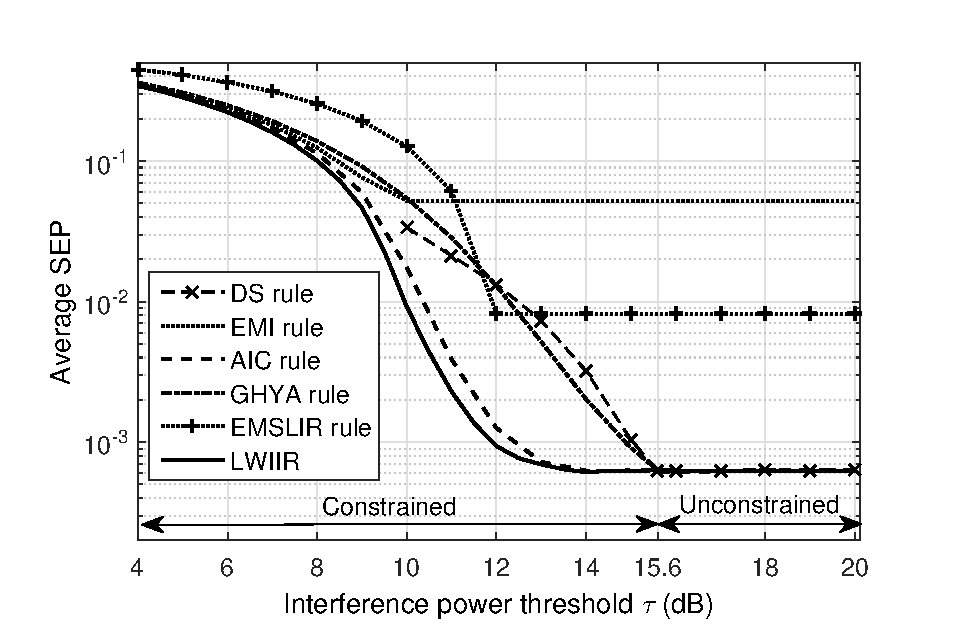
\includegraphics[width=\linewidth]{plots/BM_gs_SEP_vs_tau_pout_10_PT_12dB_Nt_4_M_4.eps}
	\caption{Performance benchmarking: Average SEPs of LWIIR and several TAS rules proposed in the literature ($\outmax = 0.1$, $\Pt = 12$~dB, $\Nt = 4$, $\Nr=1$, and QPSK).}
	\label{fig:BM_SEP_vs_tau}
\end{figure}


{\em Impact of Imperfect CSI:} Figures~\ref{fig:out_vs_tau_imp_CSI} and~\ref{fig:sep_vs_tau_imp_CSI} show the impact of imperfect CSI on the interference-outage probability and the average SEP of LWIIR as a function of $\tau$. The scenarios with imperfect $\Hmx$ ($\hpilotpower=5$~dB and $\gpilotpower\tendsto\infty$) and imperfect $\g$ ($\hpilotpower\tendsto\infty$ and $\gpilotpower=5$~dB) are compared with the perfect CSI scenario. We observe that simulation results are in agreement with the analysis in all cases in both figures. (i)~In the interference-outage constrained region ($\itau<13.6$~dB), the interference-outage probability with perfect CSI is exactly $\outmax=0.1$. However, with imperfect $\g$, the interference-outage probability always exceeds  $\outmax$ because the probability of selecting an outage-incompatible antenna increases. This also results in a  lower average SEP compared to that for perfect CSI. Interestingly, the trends are different for the imperfect $\Hmx$ scenario. Here, the interference-outage probability is below $\outmax$ for $\itau\leq10.6$~dB, and above $\outmax$ for $\itau>10.6$~dB. Another difference is that the average SEP is always worse compared to the perfect CSI scenario. (ii)~In the interference-outage unconstrained region ($\itau \geq 13.6$~dB),  
the interference unconstrained rule $\caluncons$ is optimal. The interference-outage probability becomes $\un$ for all the three cases, and it decreases exponentially as $\itau$ increases. Thus, in this region, imperfect CSI does not impact the interference-outage probability. We also see that the average SEP with imperfect $\g$ saturates to the same value as that for perfect CSI. However, with imperfect $\Hmx$, it saturates to a higher value. %Thus, in this region the average SEP saturation value depends only on the quality of the STx-SRx channel.  

\begin{figure}
	\centering
	 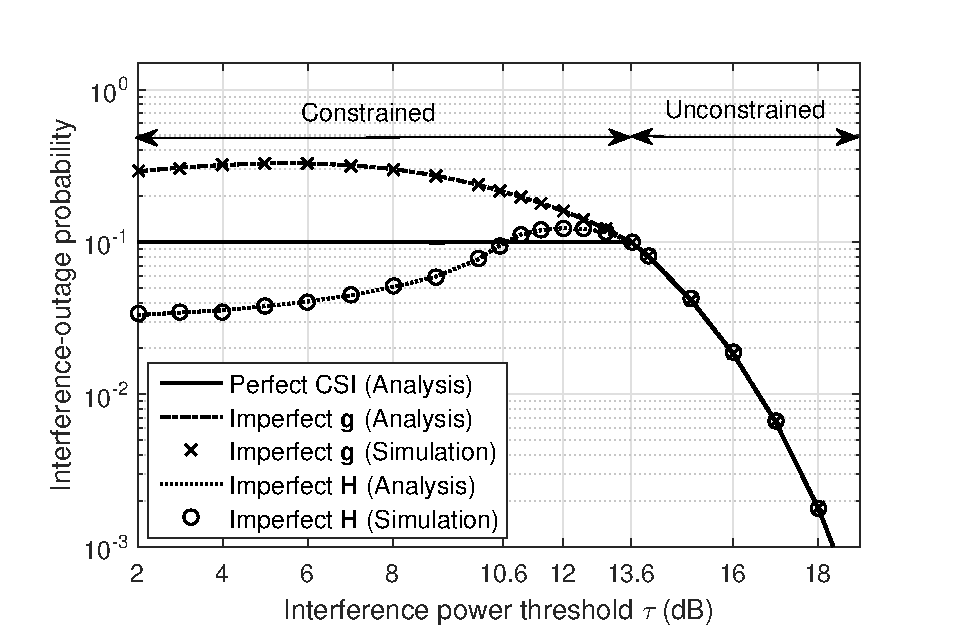
\includegraphics[width=\linewidth]{plots/Combined_outage_vs_tau_pout_10_PT_10dB_Nt_2_Nr_2_M_4.eps}
	\caption{Imperfect CSI: Interference-outage probability as a function of $\itau$ ($\outmax=0.1$, $\Pt = 10$~dB, $\Nt = 2$, $\Nr = 2$, and QPSK).}
	\label{fig:out_vs_tau_imp_CSI}
\end{figure}


\begin{figure}
	\centering 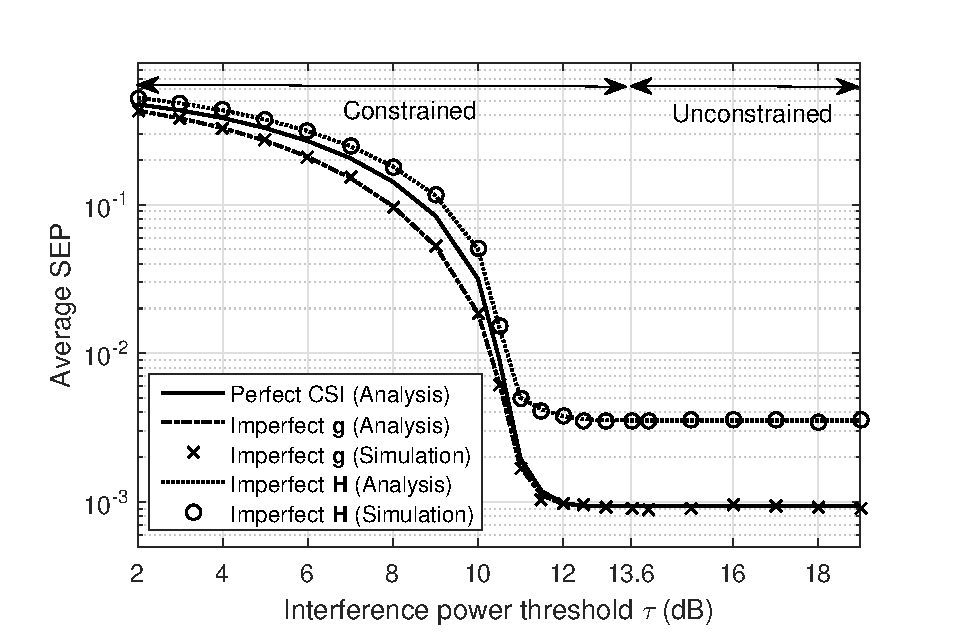
\includegraphics[width=\linewidth]{plots/Combined_SEP_vs_tau_pout_10_PT_10dB_Nt_2_Nr_2_M_4.eps}
	\caption{Imperfect CSI: Average SEP as a function of $\itau$ ($\outmax=0.1$, $\Pt = 10$~dB, $\Nt = 2$, $\Nr = 2$, and QPSK).}
	\label{fig:sep_vs_tau_imp_CSI}
\end{figure}




\section{Conclusions}
\label{sec:conclusions}
We proposed a novel and SEP-optimal TAS rule called LWIIR for an interference-outage constrained underlay CR for a general class of continuous fading models and for many constellations. The interference-outage constraints generalized the widely studied peak interference constraint. LWIIR was a discontinuous function of the STx-PRx channel power gain and was different from the TAS rules existing in the literature. We derived a general expression for the average SEP of LWIIR for an arbitrary number of transmit and receive antennas. We showed that LWIIR provides a significant performance gain compared to the other TAS rules considered in the literature. Furthermore, we saw that imperfect CSI of the STx-SRx channel power gains and that of the STx-PRx channel power gains had different effects on the interference-outage probability and the average SEP.  Incorporating multiple primary receivers, antenna subset selection, and power adaptation to make better use of the available CSI are interesting avenues for future work.

\appendix
\subsection{Proof of Lemma~\ref{lem:outage_Nt}}
\label{proof:outage_Nt}
We first derive the expression for $\outlam = \prob{\gkgrtaubypt{s}}$ in~\eqref{eq:pr_outage_ccdf}. $\Pt \gk{s}$ can exceed  $\itau$ only when $s\neq0$. Thus, using the law of total probability, $\outlam$ is given by
%
\newcommand{\eqidx}{j}
\begin{equation}
\outlam =  \sum_{\eqidx=1}^{\Nt}\text{Pr}\brac{s=\eqidx,\gk{\eqidx}>\taubypt}=\Nt\text{Pr}\brac{s=1,\gk{1}>\taubypt}.
\label{eq:out_1}
\end{equation}
%
The second equality above follows due to symmetry.

Let $k$ antennas out of the antennas $2,\ldots,\Nt$ be outage-compatible. The total number of ways in which such $k$ antennas can be chosen is $\nck{\Nt-1}{k}$. Given $k$, all these combinations are equally likely as the STx-PRx channels are i.i.d. One such combination is when the antennas $2,\ldots,k$ are outage-compatible. For it, define the event   $\setAk=\left(\gklttaubypt{2}\right)\cap\cdots\cap\left(\gklttaubypt{k+1}\right)\cap\left( \gkgrtaubypt{k+2}\right)\cap\cdots\cap\left(\gkgrtaubypt{\Nt}\right)$. Therefore, using the law of total probability, we can write $\outlam$ in~\eqref{eq:out_1} as
%
\begin{align}
\outlam &=\Nt\sum_{k=0}^{\Nt-1}\nck{\Nt-1}{k} \text{Pr}\brac{s = 1,\gk{1}>\taubypt,\setAk}, \\
&=\Nt\sum_{k=0}^{\Nt-1}\nck{\Nt-1}{k}  \text{Pr}\brac{\setGk} \text{Pr}\brac{s = 1\Given \setGk},
\label{eq:out_3}
\end{align}
%
where $\setGk$ denotes the event  $\left(\gkgrtaubypt{1}\right)\cap\setAk $. As $\gk{1},\ldots,\gk{\Nt}$ are i.i.d., we get $\prob{\setGk} = \left(1-\un\right)^k\un^{\Nt-k}$.
%where $\setGk$ denotes the event  $\left(\gkgrtaubypt{1}\right)\cap\setAk $. As $\gk{k}$ s are i.i.d., we get $\prob{\setGk} \!= \left(1-\un\right)^k\un^{\Nt-k}$.
%

{\em Expression for $\prob{s = 1\Given\setGk}$:} Given $\setGk$, $\callamrule$ in~\eqref{eq:lam_weight_rule} selects antenna 1 if $\ykplambym{1}<\yk{i}$, for $2\leq i \leq k+1$,  $\ykplambym{1}<\ykplambym{j}$, for $k+2\leq j \leq \Nt$, and $\ykplambym{1}<\yk{0}=1$. Hence,
%
\begin{align}
\label{eq:out_5}
\!\!\!\prob{s = 1\Given \setGk }&\!=\!{\bf{E}}_{\yk{1}}\!\left[\prob{s = 1\Given\setGk,\yk{1}=x}\right] ,\\
\label{eq:out_51}
&\!=\!{\bf{E}}_{\yk{1}}\!\left[\text{Pr}\left(\xplambym < 1, \xplambym<\yk{2}, \dots ,\xplambym<\yk{k+1},\right.\right.\nonumber\\
&\quad\quad\quad\quad\quad\left.\left.
\xplambym<\ykplambym{k+2}, \dots ,\xplambym < \ykplambym{\Nt}\Given\setGk,\yk{1}=x\right)\right]\!.
\end{align} 
%

Conditioning on $\yk{1}$, the events in~\eqref{eq:out_51} are mutually independent. Furthermore, $\yk{2},\ldots,\yk{\Nt} $ are identically distributed. Hence, we get
%
%\begin{multline}
%\text{Pr}\brac{s=1\Given \setGk, \yk{1}=x} = \indic{x<1-\lambym}\left[\text{Pr}\brac{\yk{2}>x+\lambym\Given\yk{1}=x}\right]^{k}\\\times \left[\text{Pr}\brac{\yk{k+2}>x\given\yk{1}=x}\right]^{\Nt-k-1}.
%\label{eq:out_6}
%\end{multline}
\begin{equation}
\text{Pr}\brac{s=1\Given \setGk, \yk{1}=x} = \indic{x<1-\lambym}\left[\text{Pr}\brac{\yk{2}>x+\lambym}\right]^{k} \left[\text{Pr}\brac{\yk{k+2}>x}\right]^{\Nt-k-1}.
\label{eq:out_6}
\end{equation}
%
Substituting this in~\eqref{eq:out_5} and writing it in terms of the CCDF and the PDF of $\yk{1}$, we get 
\begin{equation}
\text{Pr}\brac{s=1\Given\setGk} =\int_{0}^{1-\lambym}\left[F_{y}^{c}\left(x+\lambym\right)\right]^k \left[F_{y}^{c}\left(x\right)\right]^{\Nt-k-1}f_{y}(x)\,dx.
\label{eq:out_7}
\end{equation}
%Multiplying~\eqref{eq:out_7} with $\prob{\setGk}$ yields the expression for  $\prob{s=1,\setGk}$. Substituting this in~\eqref{eq:out_3} and simplifying yields~\eqref{eq:pr_outage_ccdf}.
Finally, substituting~\eqref{eq:out_7} and $\prob{\setGk}$ in~\eqref{eq:out_3} yields the interference-outage expression in~\eqref{eq:pr_outage_ccdf}. 

{\em Existence of $\lam$}: From~\eqref{eq:pr_outage_ccdf}, we see that for the class of continuous fading models, $\outlam$ is a continuous and strictly decreasing  function in $\lam$. %From~\eqref{eq:pr_outage_ccdf}, we see that for the class of continuous fading models, $\outlam$ is an integral of a continuous and strictly decreasing function in $\lam$. % Therefore, $\outlam$ is a continuous and strictly monotonically decreasing function of $\lam$. 
Furthermore, $\outlam=\un$ when $\lam=0$ and $\outlam=0$ when $\lam=\cone$. Thus, by the intermediate value theorem, for every $0\leq\outmax\leq\un$,  there exists a corresponding unique $\lam\in[0,\cone]$ such that $\outlam=\outmax$. 
  

		

\subsection{Proof of Result~\ref{thm:selection_rule_on_off}}
\label{proof:selection_rule_on_off}
In order to prove that $\callamstarrule$ is optimal, we introduce the following terminology. First, we define a feasible selection rule to be a rule that satisfies the interference-outage constraint in~\eqref{eq:cons}. Let $\F$ denote the set of all feasible rules. It is non-empty as the TAS rule that always selects antenna zero has an interference-outage probability of zero, and is, therefore, feasible.  We consider the two cases $\outmax\geq\un$ and $0\leq\outmax<\un$ separately below.

{ 1. $\outmax\geq\un$:} From the discussion in Comment a in Section~\ref{sec:LWIIR_prop}, it follows that the interference unconstrained rule $\caluncons$ is feasible and is clearly the optimal TAS rule. 

{2. $0\leq\outmax<\un$:} Here, $\caluncons$ is not feasible. Therefore, it cannot be optimal.  Instead, consider the TAS rule $\callamstarrule$, where $\lamstar$ is chosen such that the interference-outage probability of $\callamstarrule$ is equal to $\outmax$. From Lemma~\ref{lem:outage_Nt}, such a choice of $\lamstar$ always exists, is unique, and is strictly positive. For a given realization of $\yk{1},\ldots,\yk{\Nt}$, and $\gk{1},\ldots,\gk{\Nt}$, let $\sstar$ be the antenna selected by $\callamstarrule$. Then, among all the selection rules in $\F$, $\callamstarrule$, by its definition in~\eqref{eq:lam_weight_rule},  minimizes $\yk{{\sstar}} + \frac{\lamstar}{\cone}\gindic{{\sstar}}$. Consider any feasible rule $\asrule\in\F$; therefore, it selects the antenna  $s=\phi(\Hmx,\g)$.\footnote{We do not denote the antennas selected by $\callamstarrule$ and $\phi$ as $s^*(\Hmx,\g)$ and $s(\Hmx,\g)$ in order to keep the notation simple.} 

From above, it follows that   
\begin{equation}
\label{eq:opt_rul_1}  
   \explow{\Hmx,\g}{\yk{{\sstar}} + \frac{\lamstar}{\cone}\gindic{{\sstar}}} \leq  \explow{\Hmx,\g}{\yk{{s}} + \frac{\lamstar}{\cone}\gindic{{s}}}.
\end{equation}
%
Substituting $\yk{i}={\SEP(\bhk{i})}/{\cone}$ (from~\eqref{eq:yi_def}) and using $\explow{\Hmx,\g}{\gindic{i}}=\prob{\gk{i}>\taubypt}$, we get
%
\begin{equation}
\label{eq:opt_rul_2}
   \explow{\Hmx,\g}{\SEP(\hsstar)} + \lamstar \, \prob{\gk{\sstar}>\taubypt} \leq  \explow{\Hmx,\g}{\SEP(\hs)} + \lamstar \, \prob{\gk{s}>\taubypt}.
\end{equation}
%
We also know that $\prob{\gk{\sstar}>\taubypt}=\outmax$. Rearranging terms, we get
%
\begin{equation}
\label{eq:ineq_3}
\explow{\Hmx,\g}{\SEP(\hsstar)} \leq \explow{\Hmx,\g}{\SEP(\hs)} + \lamstar \left( \prob{\gk{s}>\taubypt} -  \outmax \right).
\end{equation}
%
Since $\phi$ is a feasible rule, we know that $\prob{\gkgrtaubypt{s}}\leq \outmax$. As $\lamstar>0$,~\eqref{eq:ineq_3} implies that $\explow{\Hmx,\g}{\SEP(\hsstar)} \leq \explow{\Hmx,\g}{\SEP(\hs)}$ for any feasible rule $\phi$. Hence, the result follows. %Thus, $\callamstarrule$ is optimal.




\subsection{Proof of Result~\ref{thm:SEP_exact_Nt_gen}}
\label{proof:SEP_exact_Nt_gen}
We start with the probability of error conditioned on $\y \define [\yk{1},\ldots,\yk{\Nt}]$  and $\g$, which we denote by $\prob{\Err \given \y,\g}$. Using the law of total probability, it can be written as
%
\begin{equation}
\prob{\Err \given \y,\g} =  \prob{s=\nx,\Err\given\y,\g} + \sum_{j=1}^{\Nt}\prob{s=j,\Err\given\y,\g}.
\label{eq:Perr_all_h}
\end{equation}
%
Furthermore, $\prob{s=k,\Err\given\y,\g}=\prob{s=k\given\y,\g}\prob{\Err\given\y,\g,s=k}$, for $0\leq k \leq \Nt$. Averaging over $\y$ and $\g$ and exploiting symmetry, $\avgSEP$ is given by
\begin{equation*}
\label{eq:avg_SEP_1}
 \avgSEP = \explow{\y,\g}{\prob{s=\nx\given\y,\g}\prob{\Err\given\y,\g,s=\nx}} + \Nt\explow{\y,\g}{\prob{s=1\given\y,\g}\prob{\Err\given\y,\g,s=1}}. 
\end{equation*}

Given $s=0$, the SEP is equal to\footnote{Instead of $c_1$, in the analysis,  we use the more accurate value of $\zerosep=1-\left( 1/M\right) $ for the SEP with zero transmit power.} $\zerosep$. Thus, $\prob{\Err\given\y,\g,s=\nx}=\SEP\left(\bhk{0}\right)=\zerosep$. Given $s=1$, the probability
of error depends only on $\sumnr\hk{i1}$. Thus, from~\eqref{eq:yi_def}, we get $\prob{\Err\given\y,\g,s=1}=\SEP\left(\bhk{1}\right) =\cone \yk{1}$. Hence,
%
\begin{equation}
\label{eq:avg_SEP_3}
\avgSEP  = \zerosep \explow{\y,\g}{\prob{s=\nx\given\y,\g}} + \Nt\cone\explow{\y,\g}{\yk{1}\prob{s=1\given\y,\g}}.
\end{equation}
%
From the law of total expectation, we know that $\explow{\y,\g}{\prob{s=\nx\given\y,\g}} = \prob{s = 0}$.
Similarly, 
\begin{equation}
\label{eq:avg_sep_3_one}
\explow{\y,\g}{\yk{1}\prob{s = 1\given \y,\g} } = \explow{\yk{1}}{\yk{1} \prob{s = 1\given \yk{1}}  }.
\end{equation}

Substituting these two results into~\eqref{eq:avg_SEP_3}, we get
%
%\begin{equation}
%\label{eq:avg_SEP_4}
$\avgSEP  = \termone + \termtwo$,
%\end{equation}
%
where $\termone=\zerosep \prob{s = 0}$ and $\termtwo=\Nt\cone \explow{\yk{1}}{ \yk{1}\prob{s = 1\given \yk{1}}}$. We now evaluate $\termone$ and $\termtwo$.

{\em First Term $\termone$:}
From~\eqref{eq:lam_weight_rule}, we know that ${s=0}$ is selected when the selection metrics of antennas $1,\ldots,\Nt$ exceed the selection metric of antenna $0$, \ie, $\yk{0}=1$, which happens only when they are all outage-incompatible. Therefore, we can write%Therefore, first term can be written as 
\begin{equation}
\termone = \zerosep\prob{\gkgrtaubypt{1},\dots,\gkgrtaubypt{\Nt}, \yk{1}\!+\!\lambym >1,\ldots,\yk{\Nt}\!+\!\lambym >1}.
\label{eq:termone_a}
\end{equation}
%
Using the fact that channels are i.i.d., and by writing the above formula in terms of the CCDFs of $\yk{1}$ and $\gk{1}$, we get the first term in~\eqref{eq:SEP_Nt_gen}.


{\em Second Term $\termtwo$}: From the law of total probability, we have 
%
\begin{equation}
\prob{s = 1\given \yk{1}} = \prob{s = 1,\gk{1}>\taubypt\Given\yk{1}}  + \prob{s = 1,\gk{1}\leq\taubypt\Given \yk{1}}. 
\label{eq:pr_s_1}
\end{equation}
%
We recall  the definition of the events $\setAk$ and   $\setGk=\left(\gkgrtaubypt{1}\right)\cap\setAk$ from Appendix~\ref{proof:outage_Nt}. Similarly, we define the event $\setLk\define\left(\gklttaubypt{1}\right)\cap\setAk $. Summing over all the events in which $k$ antennas out of the antennas $2,\ldots,\Nt$ are outage-compatible, we get the following in a manner similar to~\eqref{eq:out_3}:
\begin{equation}
\prob{s = 1\given \yk{1}} \! =\! \sum_{k=0}^{\Nt-1}\!\!\nck{\Nt-1}{k}\!\! 
\left[ \prob{s = 1 \Given \setGk , \yk{1}} \prob{\setGk} +  \prob{s = 1 \Given \setLk, \yk{1}} \prob{\setLk}\right].\!\! 
\label{eq:pr_s_1_2}
\end{equation}
% 
%Applying the chain rule, and using the fact that the STx-PRx channels are independent of $\yk{1}$, we get
%\begin{align} 
%\label{eq:prgrtaubypt}
%\prob{s = 1,\gkgrtaubypt{1},\setAk\Given \yk{1}} &= 
%\prob{s = 1\Given\gkgrtaubypt{1},\setAk, \yk{1}} \prob{\gkgrtaubypt{1},\setAk},\\  
%\prob{s = 1,\gklttaubypt{1},\setAk\Given \yk{1}} &= \prob{s = 1\Given \gklttaubypt{1},\setAk,\yk{1}}\prob{\gklttaubypt{1},\setAk}.
%\label{eq:prlttaubypt}
%\end{align}
%
The expression for $\prob{s = 1\given \setGk, \yk{1}}$ is given in~\eqref{eq:out_6}.  The expression for $\prob{s = 1\given \setLk, \yk{1}}$ can be derived along lines similar to that for $\prob{s = 1\given \setGk, \yk{1}}$ in~\eqref{eq:out_6}. This yields   
\begin{equation}
\text{Pr}\brac{s =1\given \setLk,\yk{1}=x} \!=\! F_{y}^{c}\brac{x}^{k}\left[\indic{x\leq\lambym} +\indic{x>\lambym}\left( F_{y}^{c}\brac{x-\lambym}\right) ^{\Nt-k-1}\right].
\label{eq:prob_gklt}
\end{equation}
%
Substituting $\prob{\setGk} = \left(1-\un\right)^k\un^{\Nt-k}$ and~\eqref{eq:out_6} in~\eqref{eq:pr_s_1_2} simplifies the first part of~\eqref{eq:pr_s_1_2}. Similarly, substituting $\prob{\setLk}=\left(1-\un\right)^{k+1}\un^{\Nt-k-1}$ and~\eqref{eq:prob_gklt} simplifies the second part of~\eqref{eq:pr_s_1_2}. Substituting~\eqref{eq:pr_s_1_2} in $\explow{\yk{1}}{ \yk{1}\prob{s = 1\given \yk{1}}}$ and averaging over $\yk{1}$ yields the~\eqref{eq:termtwo_gen}. 


\subsection{Brief Proof of Result~\ref{thm:avg_SEP_imperfect}}
\label{proof:avg_SEP_imperfect_CSI}
The antenna $s$ selected by $\callamrule$  now depends on $\yhatvec\define\left[\ykhat{1},\ldots,\ykhat{\Nt} \right]$ and $\ghatvec\define\left[\gkhat{1},\ldots,\gkhat{\Nt} \right]$, while the SEP using the antenna $k$ is given by $\cone\yk{k}$, for $1\leq k\leq\Nt$.  Hence, to analyze the average SEP, we instead condition the error probability on $\y$, $\yhatvec$, and $\ghatvec$ as follows:
%
\begin{equation}
\prob{\Err \given \y,\yhatvec,\ghatvec} =  \prob{s=\nx,\Err\given \y, \yhatvec,\ghatvec} + \sum_{k=1}^{\Nt}\prob{s=k,\Err\given\y,\yhatvec,\ghatvec}.
\label{eq:Perr_all_imp_csi}
\end{equation}  
%
Simplifying further in a manner similar to the steps from~\eqref{eq:Perr_all_h} to~\eqref{eq:avg_sep_3_one} in Appendix~\ref{proof:SEP_exact_Nt_gen}, we get
%
\begin{equation}
\label{eq:avg_SEP_3_IMP_CSI}
\avgSEP = \zerosep \prob{s=\nx} + \Nt\cone\explow{\yk{1},\ykhat{1}}{\yk{1}\prob{s=1\given \ykhat{1}}}.
\end{equation}
%

The first term in~\eqref{eq:avg_SEP_3_IMP_CSI} can be obtained by replacing $\gk{k}$ with $\gkhat{k}$ and $\yk{k}$ with $\ykhat{k}$ in~\eqref{eq:termone_a}. The expectation in the second term can be written in terms of the joint PDF $f_{\yk{1},\ykhat{1}}\left(\cdot,\cdot\right)$ of the correlated RVs $\yk{1}$ and $\ykhat{1}$ as follows:
%
\begin{equation}
\label{eq:avg_SEP_4_IMP_CSI}
\explow{\yk{1},\ykhat{1}}{\yk{1}\prob{s=1\given \ykhat{1}}}= \int_{\xhat=0}^{1} \prob{s=1\given \ykhat{1}=\xhat} \left[ \int_{x=0}^{1} x  f_{\yk{1},\ykhat{1}}\left(x,\xhat\right)\,dx\right] \,d\xhat.
\end{equation}
%
The expression for $\prob{s=1\given\ykhat{1}=\xhat}$ can be derived along lines similar to the steps from~\eqref{eq:pr_s_1} to~\eqref{eq:prob_gklt} in Appendix~\ref{proof:SEP_exact_Nt_gen}, by replacing $\yk{1}$ with $\ykhat{1}$ and $\gk{1}$ with $\gkhat{1}$. Thus, its final expression is obtained by replacing $\ccdfyrv{\cdot}$ with $\ccdfyhatrv{\cdot}$ and $\un$  with $\unhat$ in the expression for  $\prob{s=1\given\yk{1}}$ in~\eqref{eq:pr_s_1_2}. 

{\em Joint PDF $f_{\yk{1},\ykhat{1}}\left(\cdot,\cdot\right)$:} Consider first the joint PDF of two bivariate gamma RVs $V\define\sumnr\hk{i1}$ and $W\define\sumnr\hkhat{i1}$, which is given by~\cite[(6.1)]{simon_alouini_book}:
\begin{equation}
\label{eq:bivargammaPDF}
f_{V,W}(v,w) = \frac{\exp\left[{-\frac{1}{(1-\rhoh)}\left( \frac{v}{\muh}+\frac{w}{\muhhat}\right) } \right]}{\Gamma\left(\Nr \right) \left(1-\rhoh \right)\muh\muhhat }\left(\frac{vw}{\rhoh \muh\muhhat}\right)^{\frac{\Nr-1}{2}}  I_{\Nr-1}\left(\frac{2\sqrt{\rhoh vw}}{(1-\rhoh)\sqrt{\muh\muhhat}}\right),~v, w \geq 0.
\end{equation}
%  
Here, $I_{\Nr-1}\left(\cdot \right) $ is the modified Bessel function of $(\Nr-1)^{\text{th}}$ order. From it, we can obtain joint PDF $f_{\yk{1},\ykhat{1}}\left(\cdot,\cdot\right)$ using the variable transformation $\yk{1}=\exp\left(-\Pt V/(\ctwo\noisevar) \right) $ and $\ykhat{1}=\exp\left(-\Pt W/(\ctwo\noisevar) \right)$ from~\eqref{eq:yi_def} and~\eqref{eq:yihat_def}, respectively.  
%
%\begin{multline}
%\label{eq:bivaratey1PDF}
%f_{\yk{1},\ykhat{1}}(x,\xhat) = \frac{1}{\Gamma\left(\Nr \right)\left(1-\rhoh \right)}\frac{\ctwo^{\Nr+1}}{\snr\snrhat} \left(\frac{\ln(x)\ln(\xhat)}{\rhoh \snr\snrhat}\right)^{\frac{\Nr-1}{2}} x^{\frac{\ctwo}{(1-\rhoh)\snr}-1 } \xhat^{\frac{\ctwo}{(1-\rhoh)\snrhat}-1 } \\ I_{\Nr-1}\left(\frac{2\ctwo}{(1-\rhoh)}\sqrt{\frac{\rhoh\ln(x)\ln(\xhat)}{ \snr\snrhat}}\right).
%\end{multline}
% 
We can then show that %$\int_{0}^{1} x f_{\yk{1}\ykhat{1}}\left(x,\xhat\right)\,dx = {\T^{\Nr}\left(-\ln\left({\xhat} \right)\right)^{\Nr-1}\xhat^{\D}}/{(\Nr-1)!}$.
\begin{equation}
\label{eq:y1_jpdf}
\int_{x=0}^{1} x f_{\yk{1}\ykhat{1}}\left(x,\xhat\right)\,dx = \frac{\T^{\Nr}\left(-\ln\left({\xhat} \right)\right)^{\Nr-1}\xhat^{\D}}{(\Nr-1)!}.
\end{equation}
Substituting this in~\eqref{eq:avg_SEP_4_IMP_CSI} and then in~\eqref{eq:avg_SEP_3_IMP_CSI}  yields~\eqref{eq:avg_SEP_imperfect}.



\subsection{Proof of Result~\ref{thm:outage_imperfect_CSI}}
\label{proof:outage_imperfect_CSI}
Instead of~\eqref{eq:out_1}, we write the outage probability as follows: 
\begin{equation}
\outlam=\Nt\text{Pr}\brac{s=1,\gk{1}>\taubypt,\gkhat{1}>\taubypt} + \Nt\text{Pr}\brac{s=1,\gk{1}>\taubypt,\gkhat{1}\leq\taubypt}.
\label{eq:outhat_2}
\end{equation}
Let $k$ be the number of STx antennas for which $\gkhatlttaubypt{j}$, for $2\leq j \leq\Nt$. Similar to the events $\setAk$, $\setLk$,  and  $\setGk$ that are defined in Appendices~\ref{proof:outage_Nt} and~\ref{proof:SEP_exact_Nt_gen}, we define $\setAkhat=\left(  \gkhatlttaubypt{2}\right)\cap\cdots\cap\left(\gkhatlttaubypt{k+1}\right)\cap\left(\gkhatgrtaubypt{k+2}\right)\cap\dots\cap\left(\gkhatgrtaubypt{\Nt}\right)$, $\setLkhat\define\left(\gkhatlttaubypt{1}\right)\cap\setAkhat$, and $\setGkhat\define\left(\gkhatgrtaubypt{1}\right)\cap\setAkhat$ for imperfect CSI. Then, along lines similar to~\eqref{eq:pr_s_1_2}, we can write~\eqref{eq:outhat_2}  as
%
\begin{multline}
\outlam =\Nt\sum_{k=0}^{\Nt-1}\nck{\Nt-1}{k}\left[ \prob{s = 1 \Given \gkgrtaubypt{1},\setLkhat} \prob{\gkgrtaubypt{1},\setLkhat} \right. \\  +\left.
\prob{s = 1 \Given\gkgrtaubypt{1}, \setGkhat } \prob{\gkgrtaubypt{1},\setGkhat}\right]. 
\label{eq:pr_s_1_2_imp}
\end{multline}
%

Consider the first term inside the summation in~\eqref{eq:pr_s_1_2_imp}. To compute it, we proceed as follows:
\begin{enumerate}
\item  Given $\gkhatlttaubypt{1}$, from the definition of $s$ in~\eqref{eq:shat}, selection of antenna 1 does not depend on $\gk{1}$. Thus, $\prob{s = 1 \Given \gkgrtaubypt{1},\setLkhat}=\prob{s = 1 \given \setLkhat}$. Its expression is obtained by replacing $\yk{1}$ with $\ykhat{1}$ and $\ccdfyrv{\cdot}$ with $\ccdfyhatrv{\cdot}$ in~\eqref{eq:prob_gklt} and then averaging over $\ykhat{1}$. 

\item Using the fact that $\gkhat{2},\ldots\gkhat{\Nt}$ are independent of $\gk{1}$ and $\gkhat{1}$, we get  
\begin{equation}
\prob{\gkgrtaubypt{1},\setLkhat} =\prob{\gkgrtaubypt{1},\gkhatlttaubypt{1}}\prob{\setAkhat}. 
\end{equation}
Furthermore, since $\gkhat{2},\ldots,\gkhat{\Nt}$ are i.i.d., we get $\prob{\setAkhat}=\left(1- \unhat \right)^{k} \unhat^{\Nt-k-1}$. We also know that 
%\begin{equation}
%\label{eq:g1_integral}
$\Probglt\define\prob{\gkgrtaubypt{1},\gkhatlttaubypt{1}}=\int_{\xhat=0}^{\tau/\Pt}\int_{x=\tau/\Pt}^{\infty}f_{\gk{1},\gkhat{1}}\left(x,\xhat \right)\,dx\, d\xhat,$
%\end{equation}
where $f_{\gk{1},\gkhat{1}}\left(\cdot,\cdot \right)$ is the joint PDF of the bivariate exponential RVs $\gk{1}$ and $\gkhat{1}$.  This is a special case of~\eqref{eq:bivargammaPDF} with $\Nr=1$, and is obtained by replacing $\muh$, $\muhhat$, and $\rhoh$ with $\mug$, $\mughat$, and $\rhog$, respectively.
%\begin{equation}
\label{eq:bivargPDF}
%f_{\gk{1},\gkhat{1}}\left(x,\xhat \right) = \frac{\exp\left[{-\frac{1}{(1-\rhog)}\left( \frac{x}{\mug}+\frac{\xhat}{\mughat}\right) } \right]}{\left(1-\rhog \right)\mug\mughat}  I_{0}\left(\frac{2\sqrt{\rhog x\xhat}}{(1-\rhog)\sqrt{\mug\mughat}}\right),~\text{for}\; x,\xhat>0.
%\end{equation}
Then, evaluating the above integral yields the expression for $\Probglt$ in the result statement.


%\begin{equation}
%\prob{\gkgrtaubypt{1},\gkhatlttaubypt{1}} =  \un Q_1\left(\frac{\rhog}{ \gpilotpower} \sqrt{\frac{2\itau}{ \gpilotpower\Pt}},\sqrt{\frac{2 \gpilotpower\itau}{\Pt}}\right)  - \frac{\unhat}{2} \left( 1 + e^{-\frac{2\itau\rhog}{ \gpilotpower\Pt}}I_{0}\left(\frac{2\itau\rhog}{ \gpilotpower\Pt} \right) \right).
%\end{equation}
\end{enumerate}

The second term inside the summation in~\eqref{eq:pr_s_1_2_imp} can be simplified in a similar manner. Substituting the expressions for these two terms in~\eqref{eq:pr_s_1_2_imp} yields~\eqref{eq:pr_outage_impefect}.
 

\bibliographystyle{IEEEtran}
%\bibliography{../../../Bibtex/bibJournalList,../../../Bibtex/standard,../../../Bibtex/sarvendra,../../../Bibtex/IEEE_papers,../../../Bibtex/mimo,../../../Bibtex/salil,../../../Bibtex/book}

\bibliography{./Bibtex/bibJournalList,./Bibtex/standard,./Bibtex/sarvendra,./Bibtex/IEEE_papers,./Bibtex/mimo,./Bibtex/salil,./Bibtex/book}

%\bibliography{../../../Bibtex/sarvendra,../../../Bibtex/IEEE_papers}


\end{document}


